\documentclass[conference, a4paper]{IEEEtran}
\IEEEoverridecommandlockouts
% The preceding line is only needed to identify funding in the first footnote. If that is unneeded, please comment it out.
\usepackage{cite}
\usepackage{amsmath,amssymb,amsfonts}
\usepackage{algorithmic}
\usepackage{graphicx}
\usepackage{textcomp}
\usepackage{xcolor}
\def\BibTeX{{\rm B\kern-.05em{\sc i\kern-.025em b}\kern-.08em
    T\kern-.1667em\lower.7ex\hbox{E}\kern-.125emX}}
\ifCLASSOPTIONcompsoc
    \usepackage[caption=false, font=normalsize, labelfont=sf, textfont=sf]{subfig}
\else
\usepackage[caption=false, font=footnotesize]{subfig}
\fi

\addtolength{\topmargin}{+0.12cm}

\columnsep 0.25in

\begin{document}

\title{Wheat Yield Forecasting using Regression Algorithms and Neural Network}
\author{\IEEEauthorblockN{ Cheng Dai}
\IEEEauthorblockA{\textit{School of Information and Communication Engineering } \\
\textit{University of Electronic Science and Technology of China}\\
Chengdu, China \\
daichengzyw@gmail.com}
\and
\IEEEauthorblockN{Yinqin Huang}
\IEEEauthorblockA{\textit{School of Information and Communication Engineering,} \\
\textit{University of Electronic Science and Technology of China}\\
Chengdu, China  \\
hyinq@hotmail.com}
\and
\IEEEauthorblockN{Minghao Ni}
\IEEEauthorblockA{\textit{School of Information and Communication Engineering} \\
\textit{University of Electronic Science and Technology of China}\\
Chengdu, China \\
845101809@qq.com}
\and
\IEEEauthorblockN{Xingang Liu*}
\IEEEauthorblockA{\textit{School of Information and Communication Engineering} \\
\textit{University of Electronic Science and Technology of China}\\
Chengdu, China \\
hanksliu@uestc.edu.cn}
}

\maketitle

\begin{abstract}
  This paper considers the crop yield forecasting problem base on the wheat yield dataset of the U.S. To provide advice for farmers to raise the per unit area yield under the circumstance that the demand for food production are significantly increasing while the cultivated land area not expanded in recent decades, we compose a Bi-LSTM model consists of 3 stacked Bi-LSTM layers to predict wheat yield and test common used regression algorithms on the same dataset which have been preprocessed including the processing of filling in the missing items, dropping abnormal data and feature selection. The result shows that the Bi-LSTM model's $R^2$ score is 0.85 which outperforms the other algorithms. This model can also avoid overfitting problem which is commonly found in other regression algorithms. 
\end{abstract}

\begin{IEEEkeywords}
  Prediction, Agricultural Yield, Random Forest, LSTM RNN
\end{IEEEkeywords}

\section{Introduction}
  The food issue has always been a hot topic and it directly affects many aspects of people's lives. With the explosive growth of the world population, countries all over the world are exploring methods to grow crops with less natural resource consumption while increasing production under the guarantee of environmental protection. In such situation, the precision and intelligence of agriculture are becoming increasingly important. Therefore, researchers have focused on the collection, combination and processing of external information such as climate, satellites and geography in recent years. Such researches may improve modern agricultural technology and also help increase agricultural yield and quality.

  The forecast of crop yield is an important part of modern agricultural technology. It can effectively predict agricultural output, which is able to help people adjust production methods in time and improve production efficiency. Many developed countries and regions have advanced agricultural yield forecasting system, such as Monitoring Agricultural Resources (MARS) of EU. MARS has been using remote sensing since 1988, which initially designed to apply the newly emerging space technologies for providing independent and timely information on crop areas and yields. 
  
  Over the past few decades, regression algorithms and sensor technologies have developed rapidly with the advancement of computing hardware and theories, which directly leads to the emergence of more accurate algorithm of prediction. At the beginning, statistical-based models with probability theory or regression methods were widely used to implement yield forecasting\cite{Matis1985, stephens1995crop}. Since the explosive development of space technology and electronic industry, remote sensing and sensor network are utilized to farmland monitoring.  The data from remote sensing and sensor network have played an important role in the improvement of the prediction accuracy\cite{You2017, Baruth}. Recent years, the raise of deep learning has also boosted the development of crop yield forecasting. Many deep learning models have been applied to this area, which allows more complicated data can be processed rather than the simple weather data. The process of this paper is shown in Fig.~\ref{fig:arch}.
  % 随着回归算法的发展,对其产生了积极的影响,然后写发展

  In this paper, we test a number of algorithms including linear regression, polynomial regression, random forest, support vector machine, gradient boosting decision tree and kernel ridge regression KNN with weather data and wheat yield from 1895 different plant locations in 2013 and 2014. Meanwhile we solve the overfitting problems to avoid abnormal high performance in prediction. A deep Bi-LSTM model which is constructed by 3 stacked LSTM layers is also applied to predict crop yield and the results are compared with conventional algorithms. Finally, we obtain the best methods to implement yield forecasting. The rest of the paper is organized as follows. Section.~\ref{sec:RW} introduces the common used data and methods in crop yield prediction. Section.~\ref{sec:fm} explains the method of data processing and presents proposed Bi-LSTM model. In Section.~\ref{sec:ex}, experiment results are revealed and we discuss its feasibility and advantages. Finally, a conclusion is given about our method and future work.

  \begin{figure*}[!htb]
    \centering
    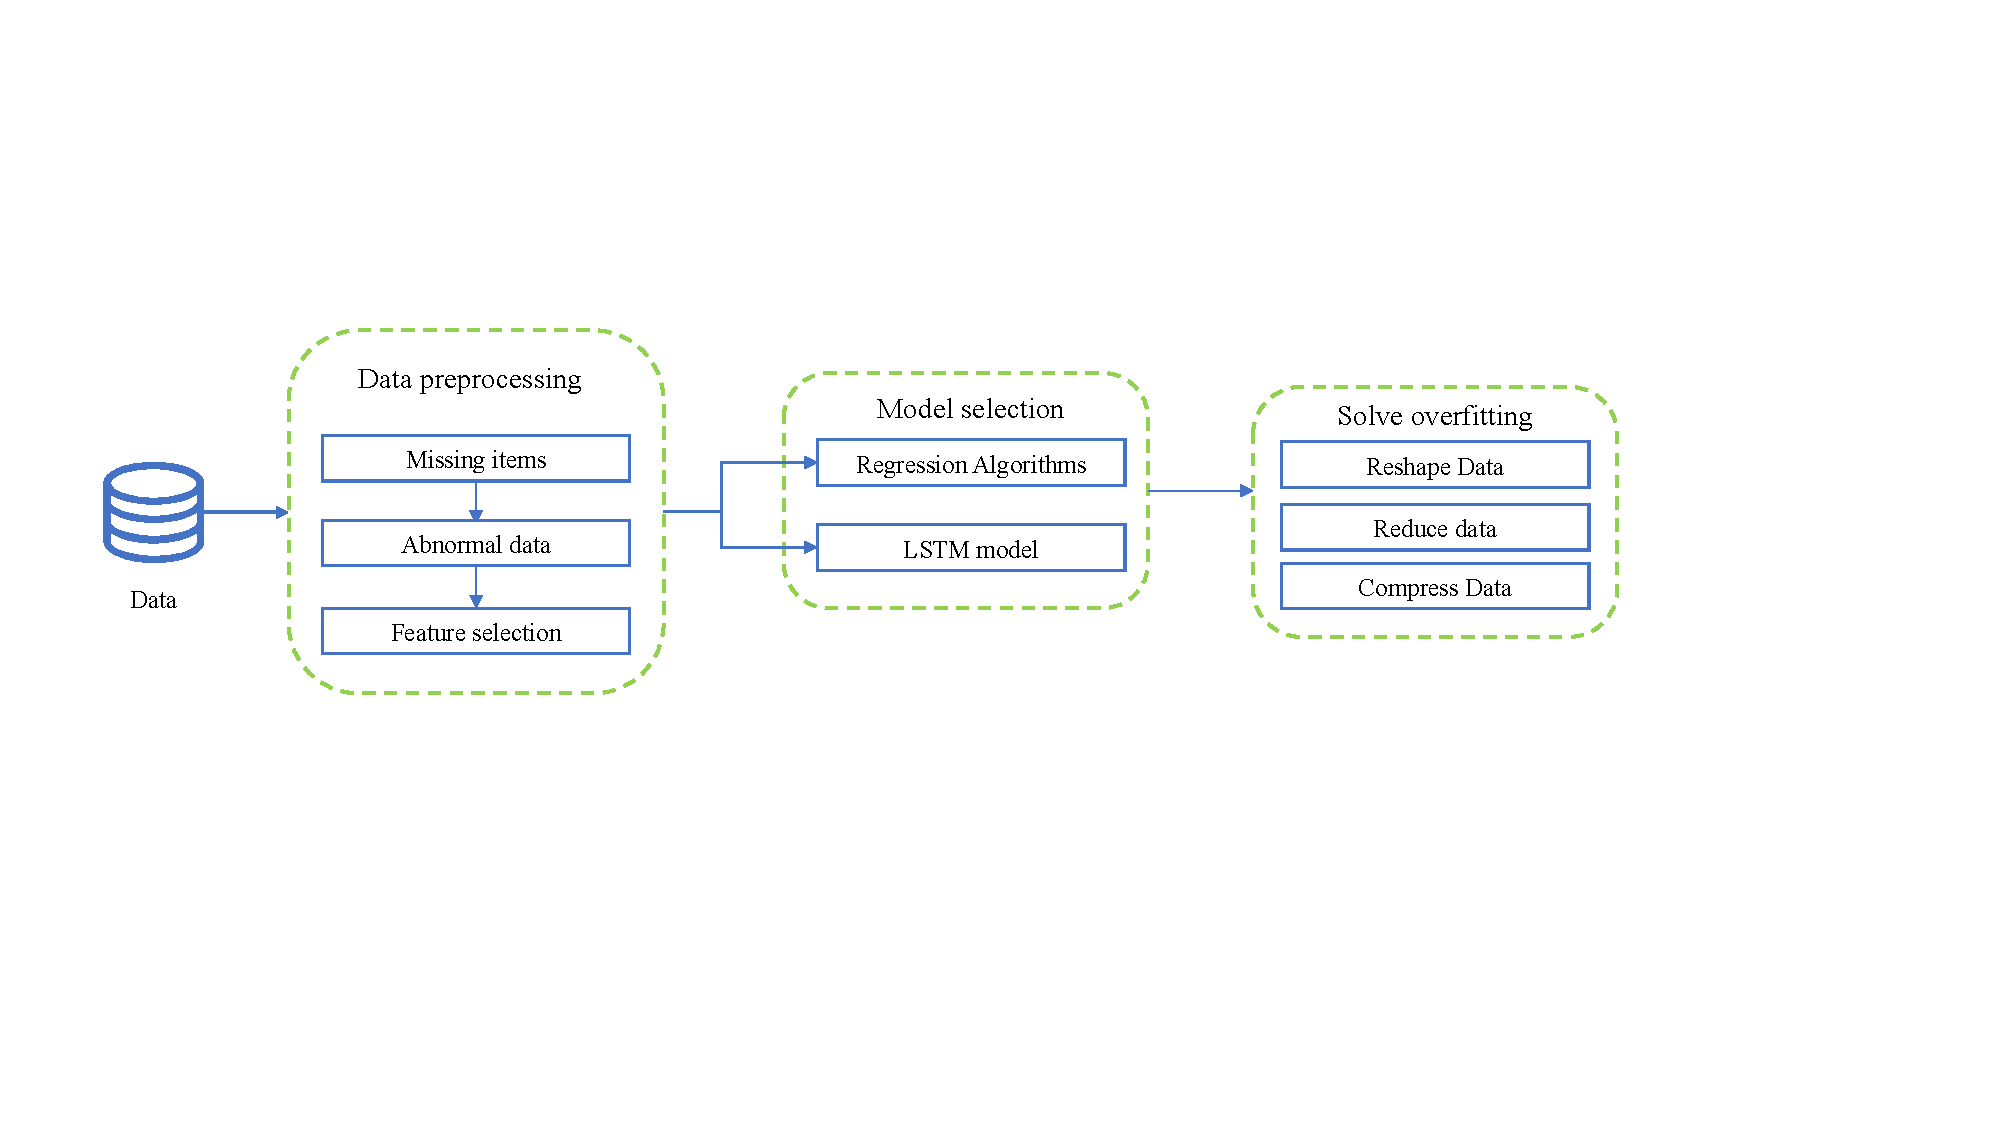
\includegraphics[width=\linewidth]{figures/arch.pdf}
    \label{fig:arch} 
    \caption{The flowchart of prediction process}
  \end{figure*}

\section{Related works} \label{sec:RW}

  \subsection{Data Resources}

    The research on crop yield forecasting mainly depends on satellite remote sensing data and sensor network data. Satellite remote sensing data are beneficial to study the relationship between crop yield and environmental conditions in the large scope while sensor network data is more used to monitor the condition within a farmland. 

    The basic idea of satellite remote sensing technology is to monitor the total energy and radiation of reflected waves from crops because the wavelength and frequency of waves are various in different growth stages. The vegetation growth situation can be obtained by observing the reflected waves on the ground through satellites, and then the yield of crops can be predicted. However, such data will be restricted by resolution of satellites and other weather factors, which results in a decrease in prediction accuracy. Bastiaanssen (2003) \cite{Bastiaanssen2003} measures crop rotation cycle and predict crop yield in Indus basin based on satellite remote sensing data. They find that this model has better prediction accuracy on wheat, rice and sugarcane comparing to cotton. Becker-Reshef (2010)\cite{Becker-Reshef2010} combines crop data with daily surface reflections data and uses a regression model to predict winter wheat yield, which can alert in time on insufficient production. De Wit (2007) \cite{DeWit2007} utilizes Kalma Filter to process the soil water content information reflected by satellite remote sensing data and experimental results illustrate that this method improves the prediction accuracy of winter wheat yield.

    Comparing to the satellite data, sensor network data are easily accessible and economical, which can provide more precise information on a small scale. Mkhabela (2011)\cite{Mkhabela2011} proposes that NDVI data can be achieved from sensors like Advanced Very High-Resolution Radiometer (AVHRR). With such data they use regression model to predict the yield of soybean and spring wheat and finally obtain high prediction metrics which controls the error below 10\%. Prasad (2006) \cite{Prasad2006} collects NDVI, Vegetation Condition index(VCI) and Temperature Condition index(TCI) data to monitor the drought condition and assess vegetation yield. According to these data, they apply piecewise linear regression method and successfully predict the soybean yield for 19 years. Therefore, sensor network data have been proved to be feasible in yield forecasting.

  \subsection{Models and Algorithms}

    The commonly utilized methods to implement crop yield forecasting are to study the impact of weather on yield. It uses agrometeorological data and put them into regression models to predict the future production. Typically, this model type is constructed by putting historical yield and agrometeorological features into a matrix, then a regression equation is applied to derive the relation between yield and features in function form. These models are simple to use and have low parameter intensiveness, but they are limited in the information they can provide outside the range of values for which the model is parameterized. USDA (2011)\cite{good2011usda} used such statistical-based regression model to forecast yield of corn in 10 major corn-producing countries. Although the method can implement yield prediction, the results are severely constrained by the data sources and it cannot involve some fatal factors to plant growth such as the patterns of cultivation, diseases or some other natural disaster.  

    In recent years, an increasing number of researchers have focused on deep learning algorithms. Deep learning models allow to input more complicated data and obtain more accurate forecasting reports. Saeed(2013)\cite{Basso2013} uses deep neural networks to predict the maize yield with a dataset containing 2267 hybrids planted in 2247 locations between 2008 and 2016. Their DNN model has a superior prediction accuracy, with 12\% root-mean-square-error (RMSE) and 50\% standard deviation of the average yield on validation datasets. You(2017)\cite{You2017} proposed a dimensionality reduction technique based on CNN or LSTM, which can automatically learn features with scarce labeled data. This algorithm incorporates a Gaussian Process component to explicitly model the spatio-temporal structure of the data and improves accuracy on the prediction of soybean yield. The experimental results verify that this model outperforms state-of-the-art algorithms.


\section{Forecasting method} \label{sec:fm}
  \subsection{Data Preprocessing} 
      The dataset includes data in winter wheat yield in the U.S with local climate conditions in 2013 and 2014, which contains 150 counties from 5 states and has 26 features, 360042 entries.

    \subsubsection{Missing items}
      There are 654 missing items in data, accounting for 1.81\% of the total data volume, among which 2013 accounts for 43.42\%. Deleting an entry with missing items may result in the decline of continuity due to the characteristics of crop growth. Filling to missing items with the nearest and most recent entry due to the continuity of climate data in both space and time. A single miss item being filled by its adjacent items, while continuous missing data can be filled from two ends to the middle one.

    \subsubsection{Abnormal data}
      By looking at the data, an apparent anomaly found in the yield. There are entries having nonzero yield with a relatively short period of time from being seeded to harvest which was recorded by column \textit{DayInSeason}.  

      Fig.~\ref{1a} shows the distribution of duration between the first record and the last in different locations, locations have 185 days of records account for 93.6\%. Therefore, delete data from locations whose planting duration less than 185 days. However, these positions not all were fully recorded for 185 days shown by Fig.~\ref{1c}, there are days not to be recorded for some reason. After all positions with miss records being deleted, all the data had consistent planting duration shown by Fig.~\ref{1d}.


      \begin{figure} 
          \centering
        \subfloat[\label{1a}]{%
            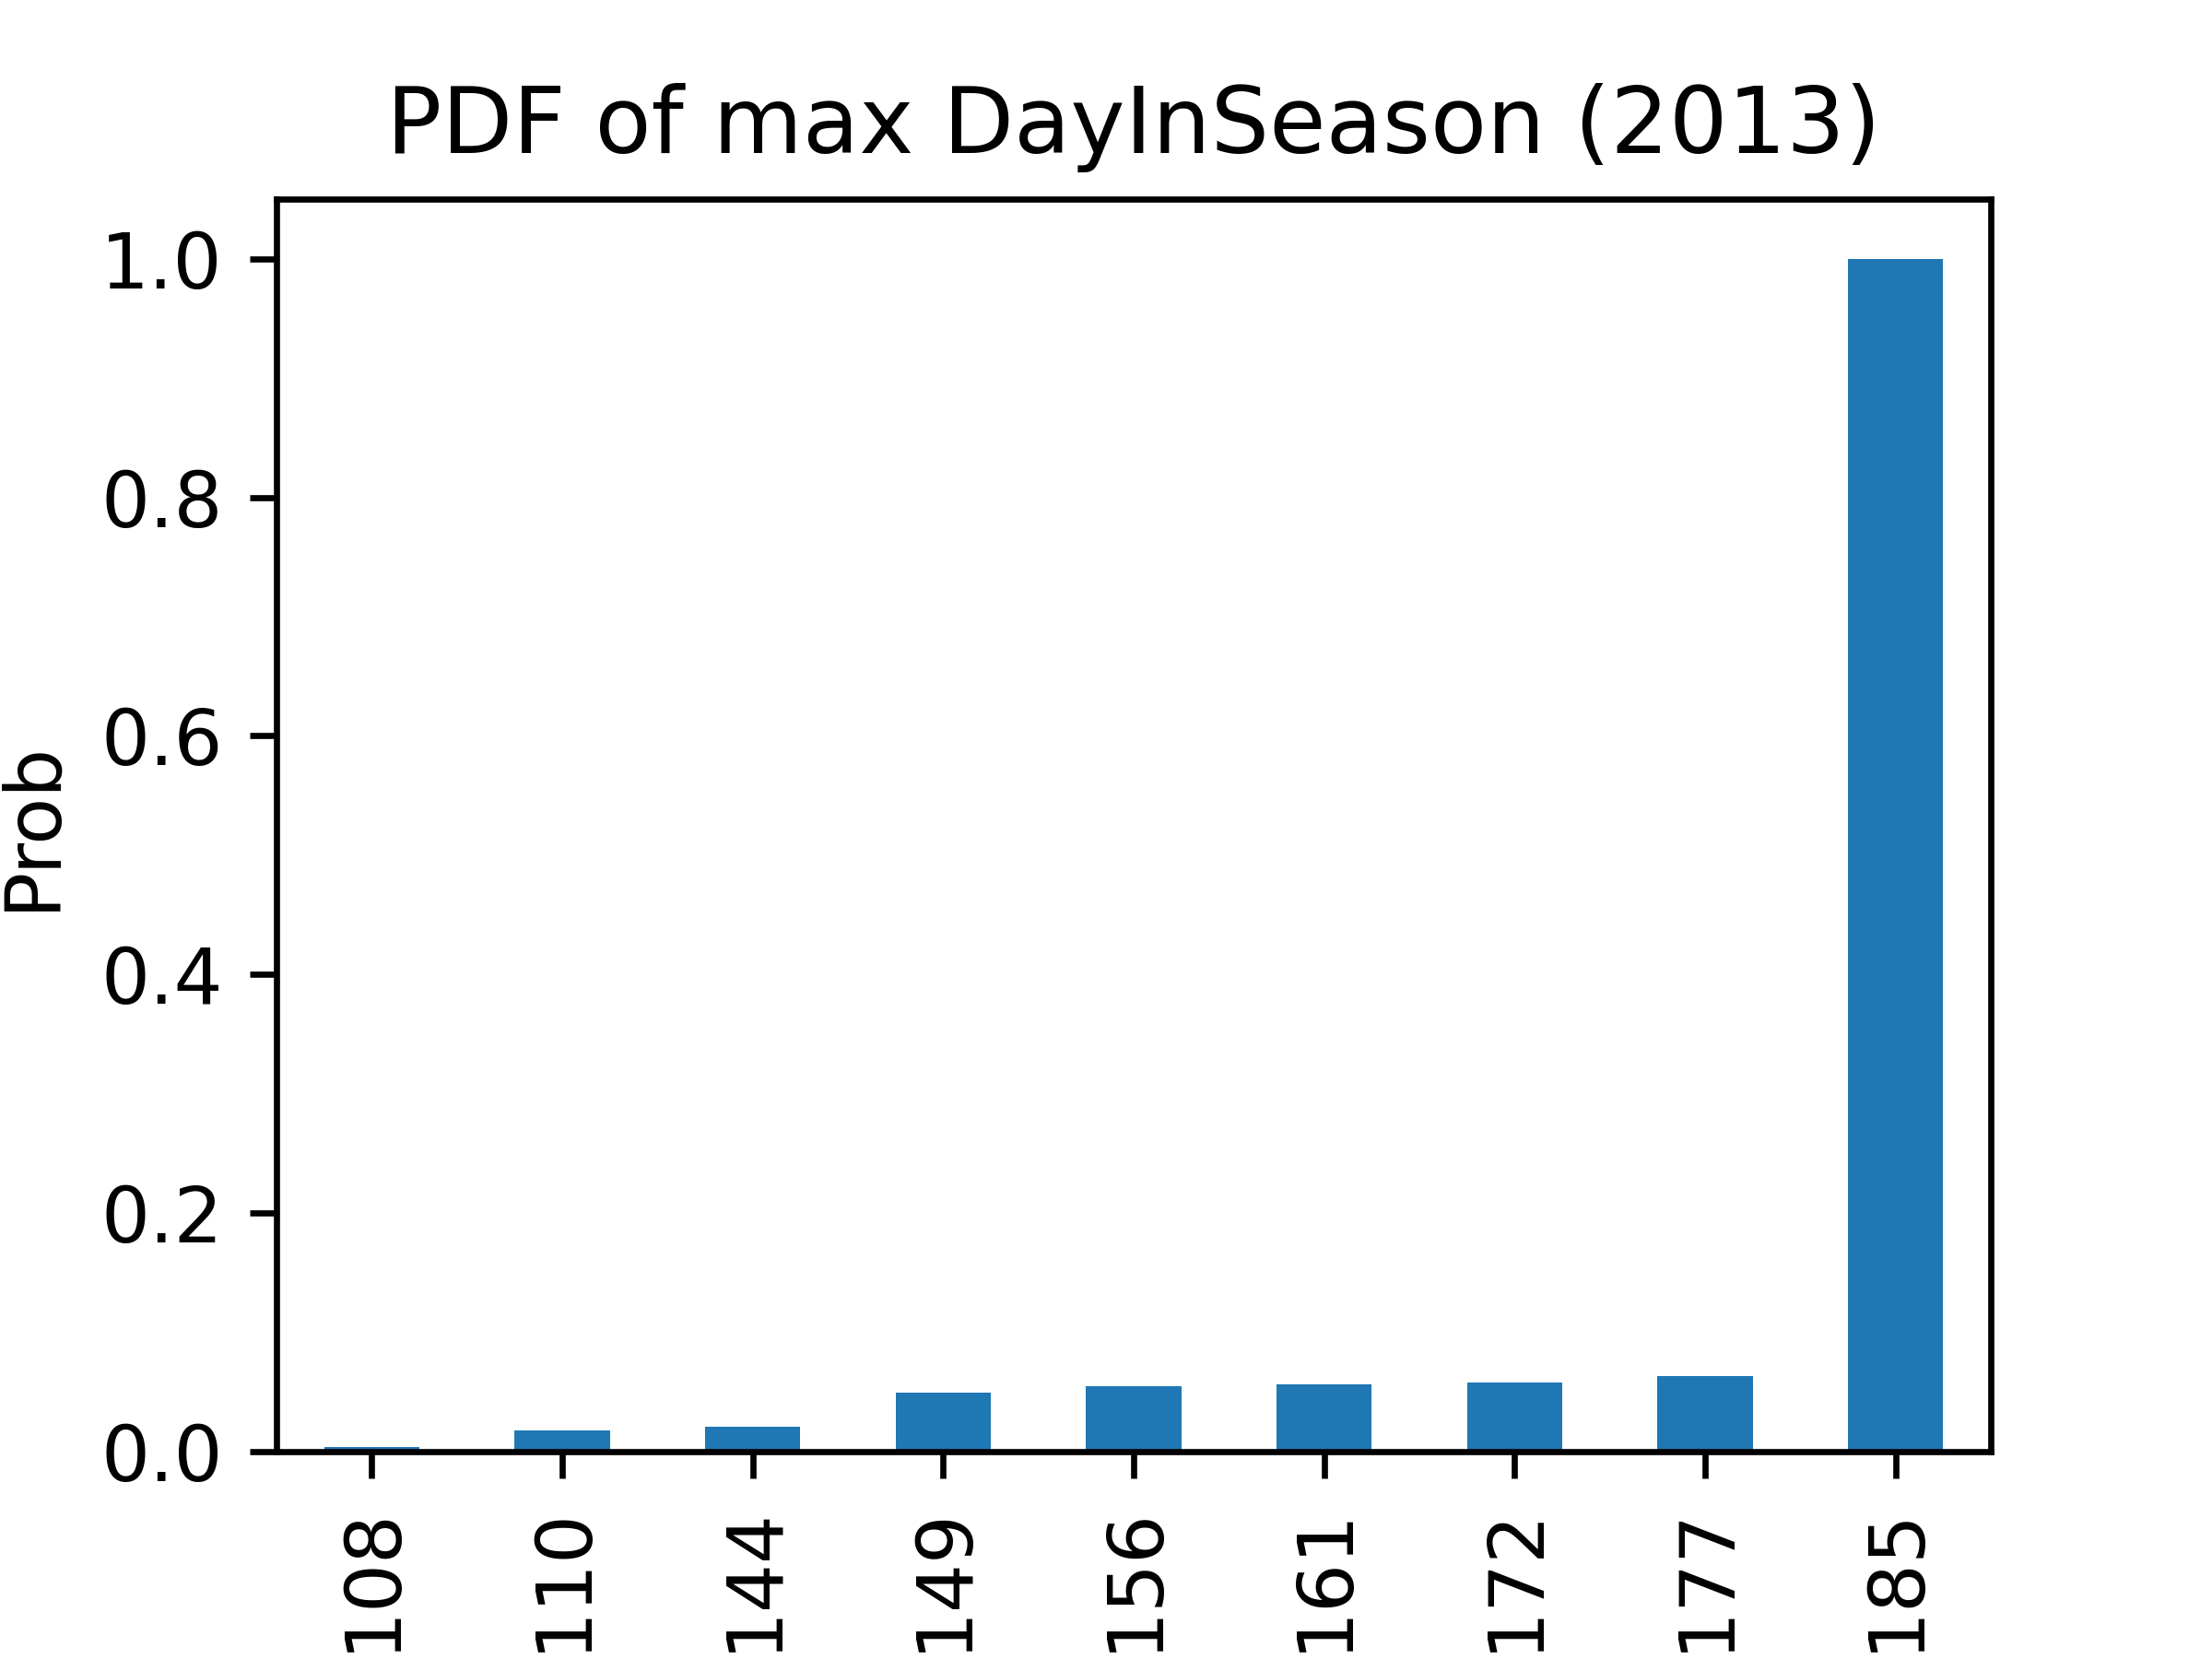
\includegraphics[width=0.45\linewidth]{./figures/PDF of max DayInSeason (2013).png}}
          \hfill
        \subfloat[\label{1b}]{%
              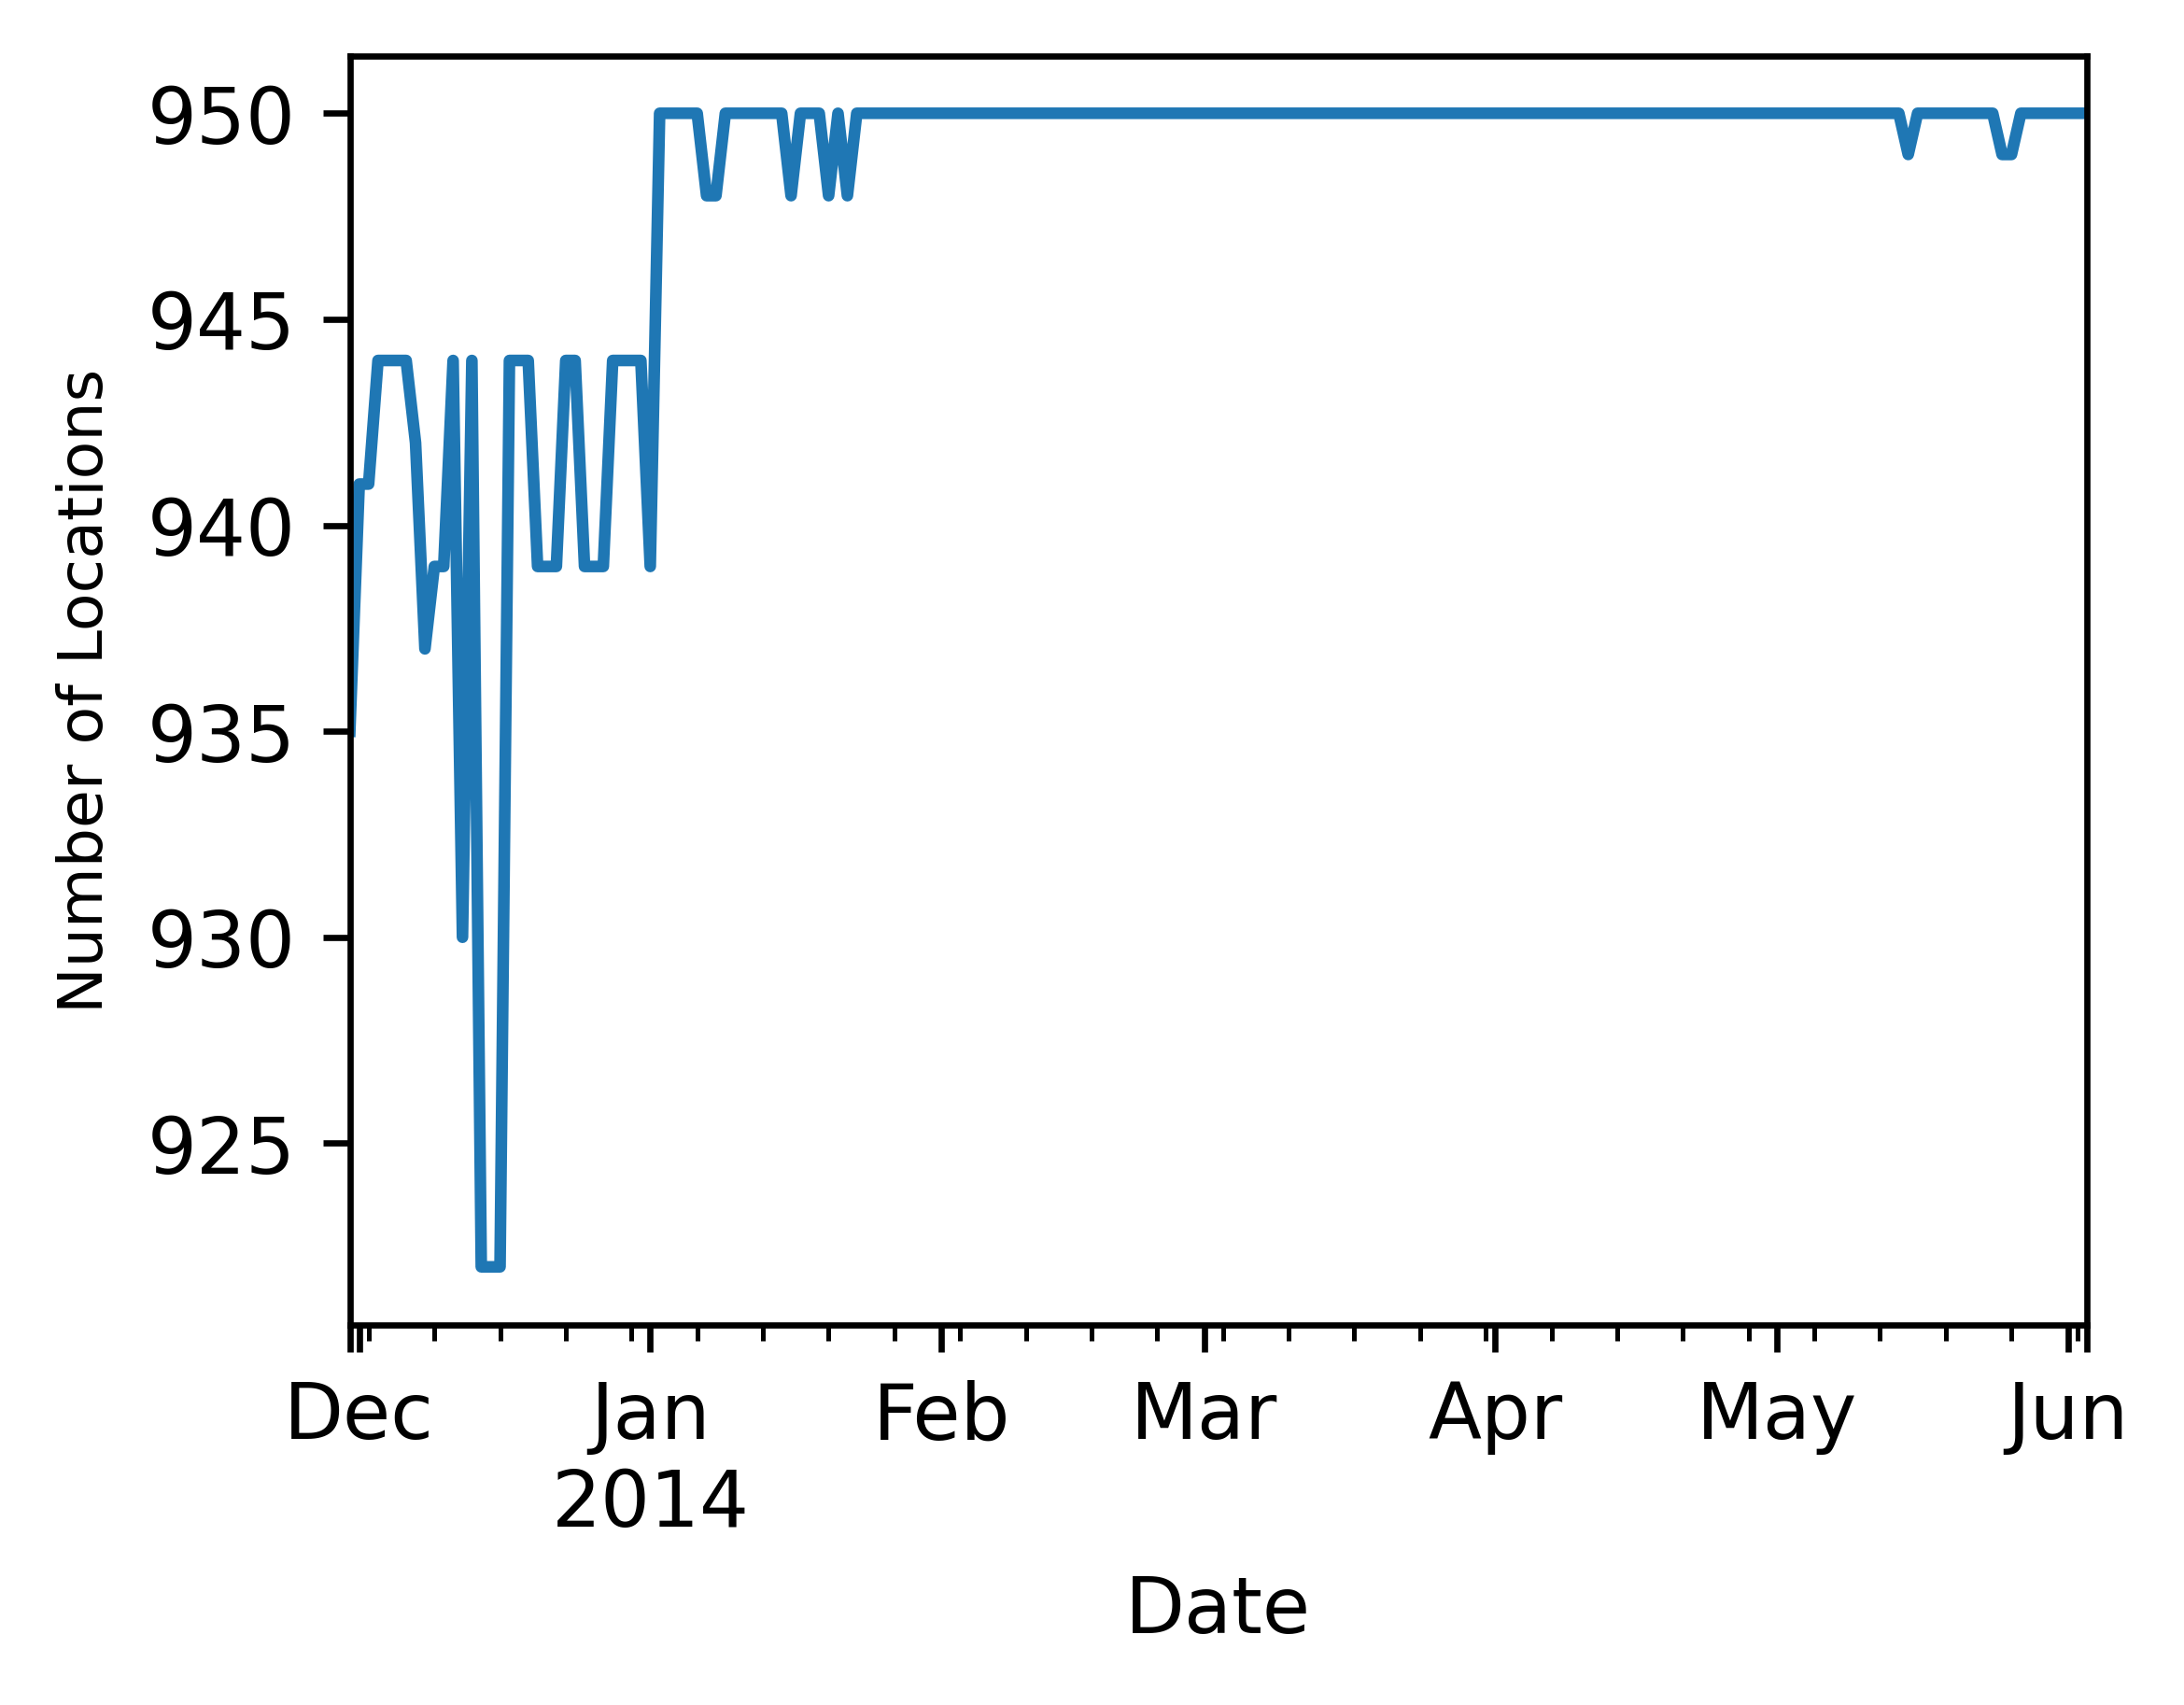
\includegraphics[width=0.45\linewidth]{./figures/date&locations(origin).png}}
          \\
        \subfloat[\label{1c}]{%
              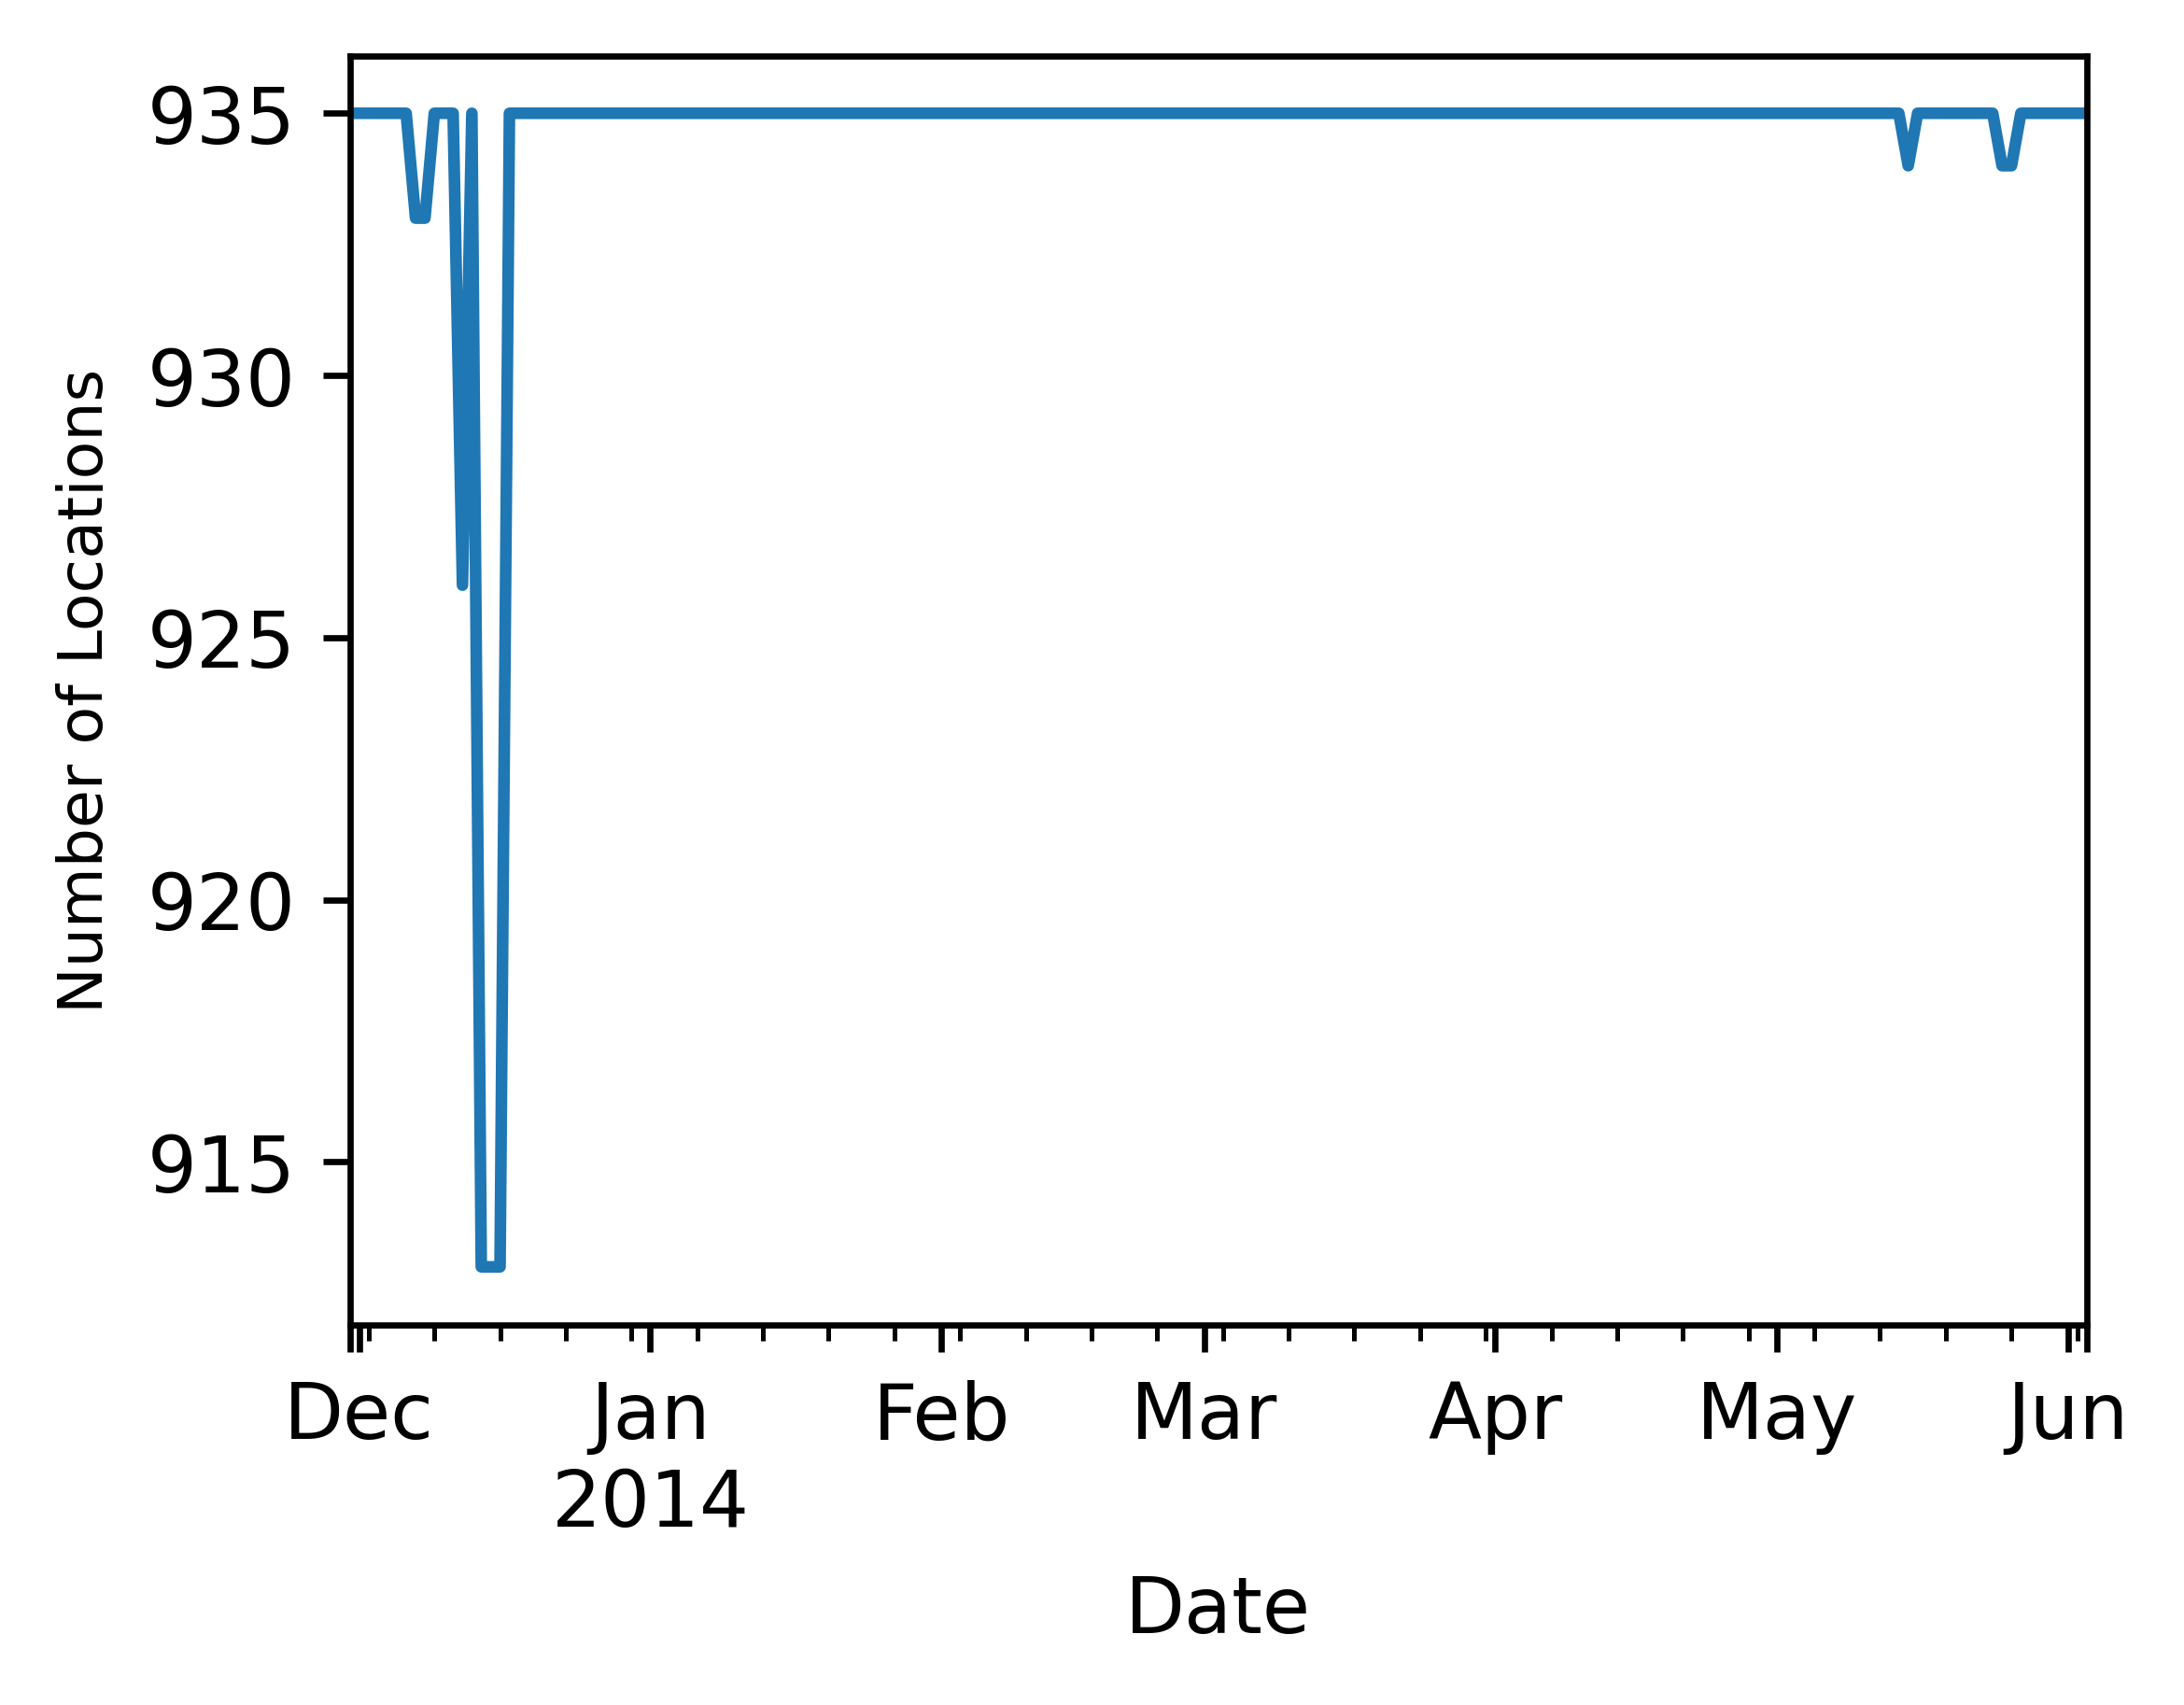
\includegraphics[width=0.45\linewidth]{./figures/date&locations.png}}
          \hfill
        \subfloat[\label{1d}]{%
              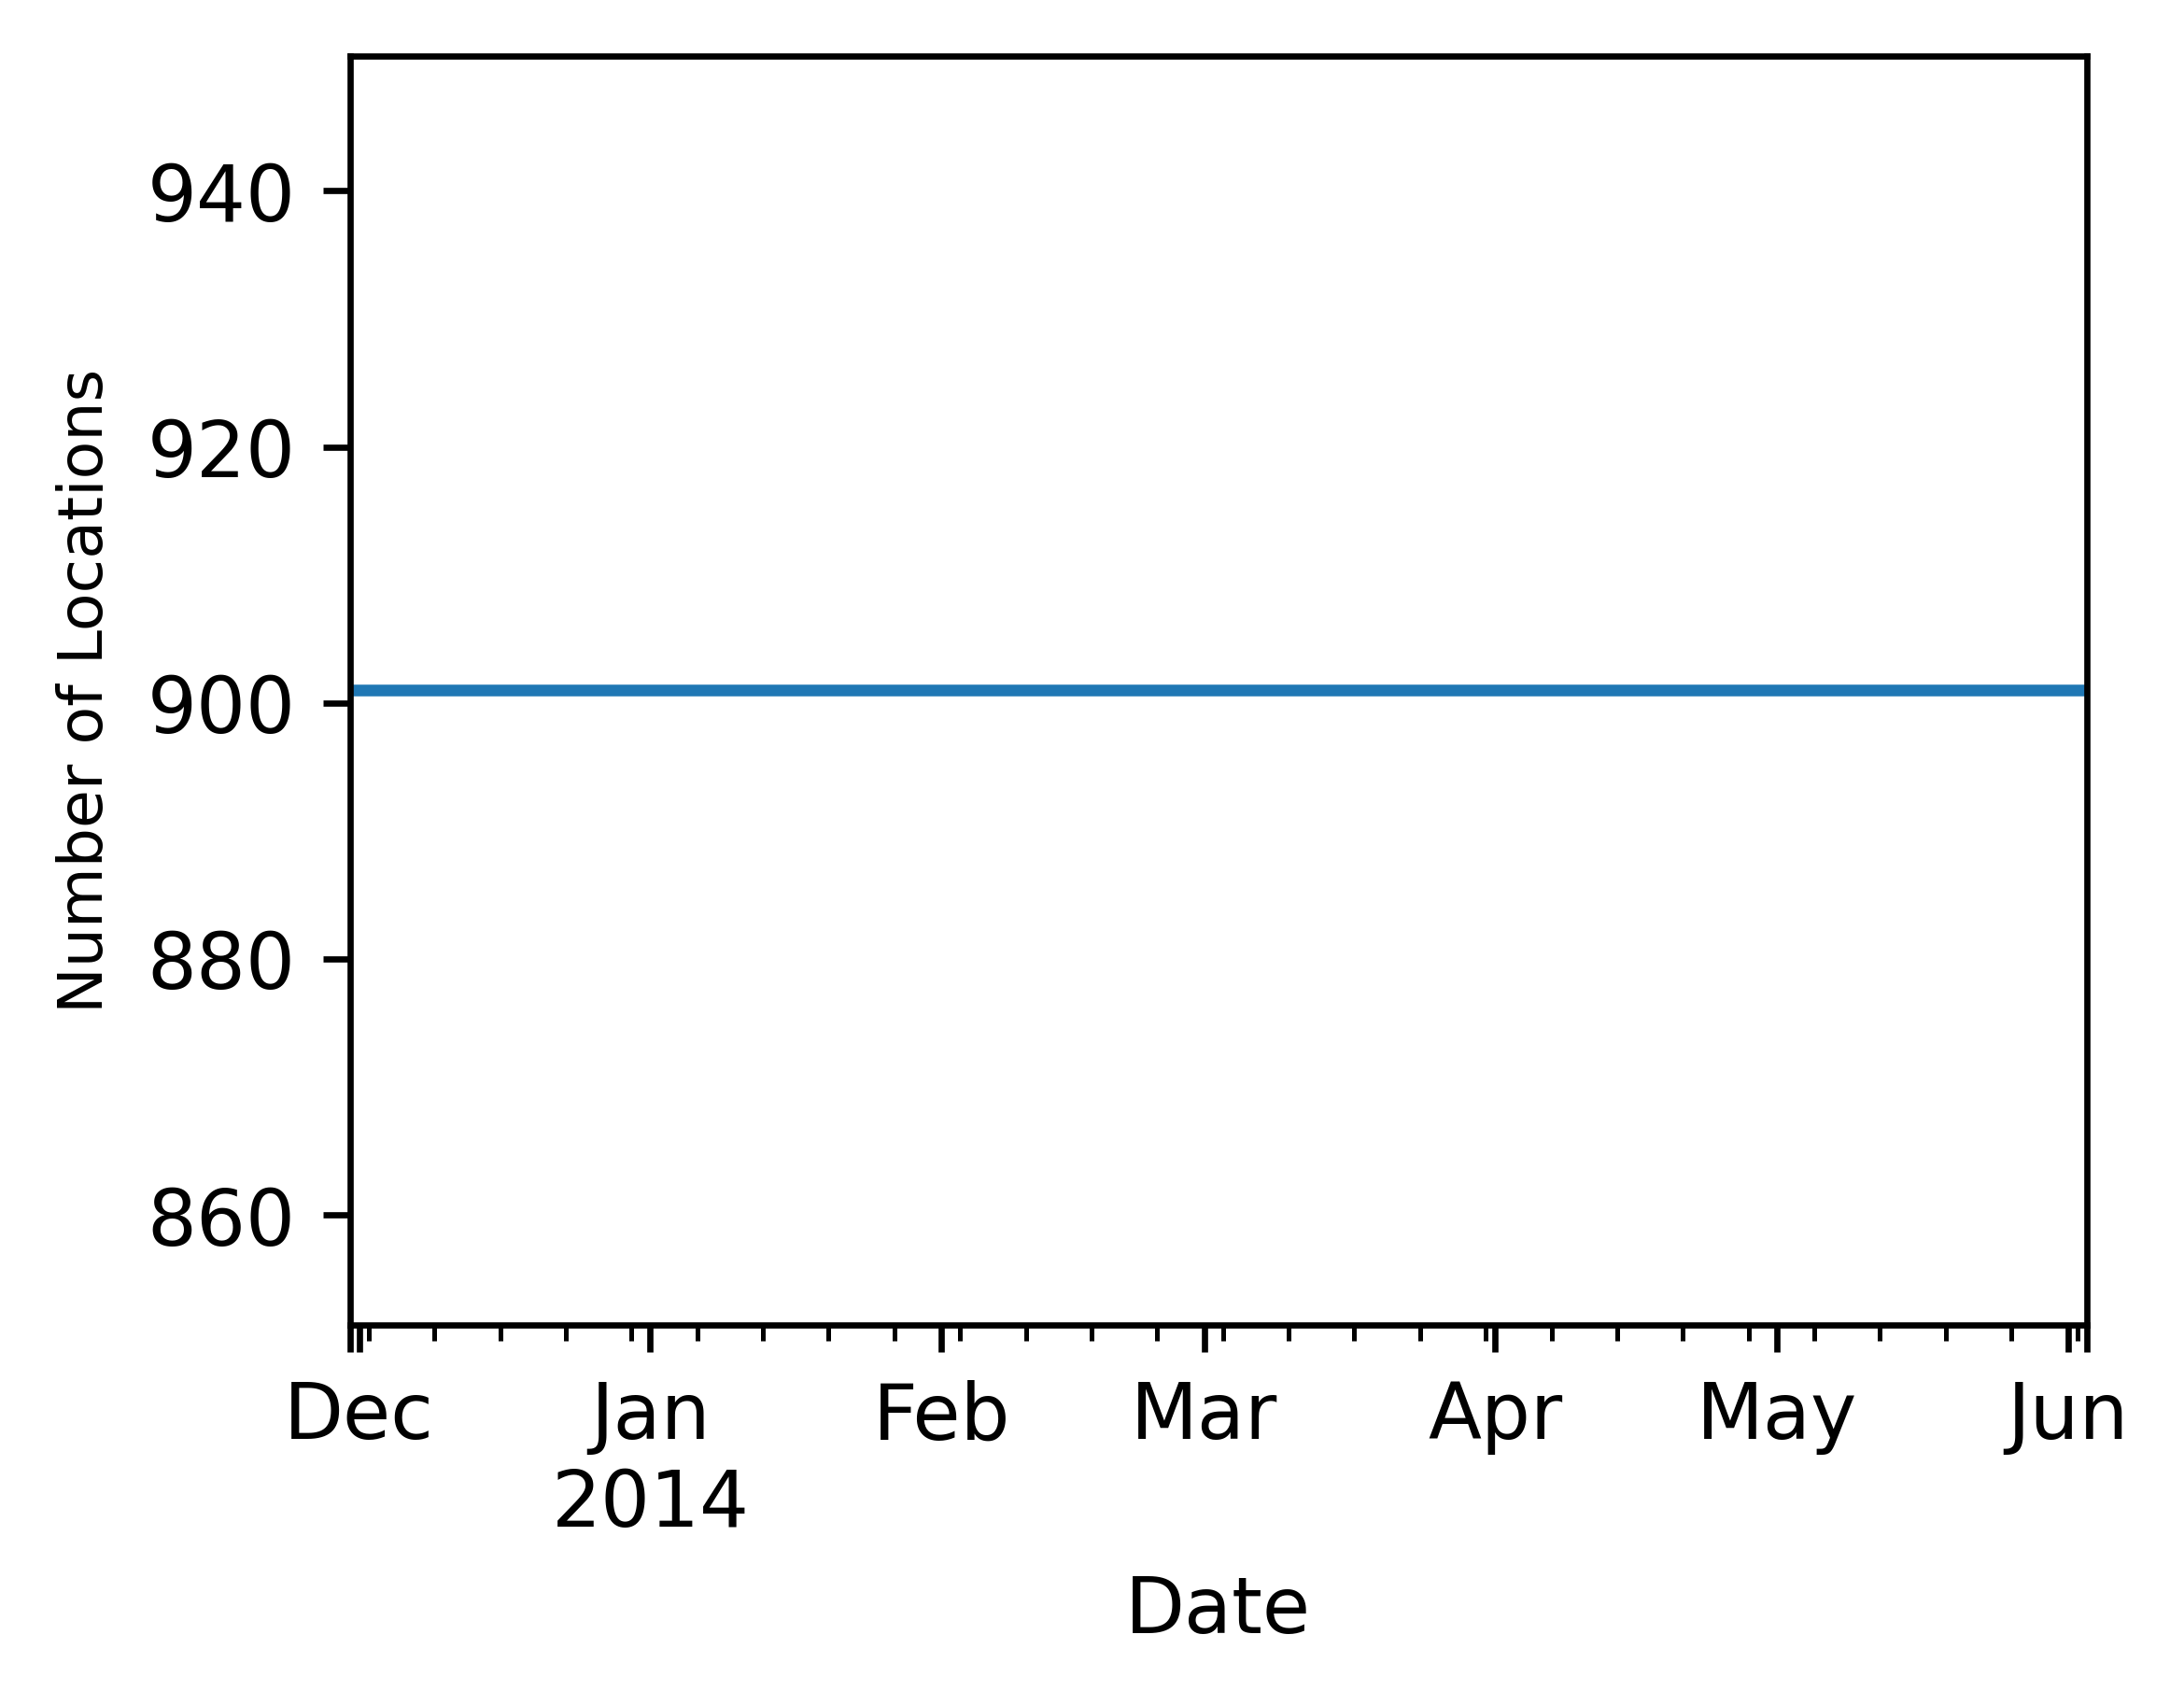
\includegraphics[width=0.45\linewidth]{./figures/date&locations(clean).png}}
        \caption{Missing data processing}
        \label{fig:missing-data} 
      \end{figure}

    \subsubsection{Map visualization}
      For data with location, map visualization can always help us find some intuitive relations between location and target. According to Fig.~\ref{fig:Map_visual}-(b), there are two intuitive conclusions:
      \begin{itemize}
          \item The yield in the northern growing areas was significantly higher than that in the south. 
          \item In the south growing areas, the more east the locations are the high the yields.
      \end{itemize}

      \begin{figure*}[!htb]
          \centering
        \subfloat[\label{mapa}]{%
            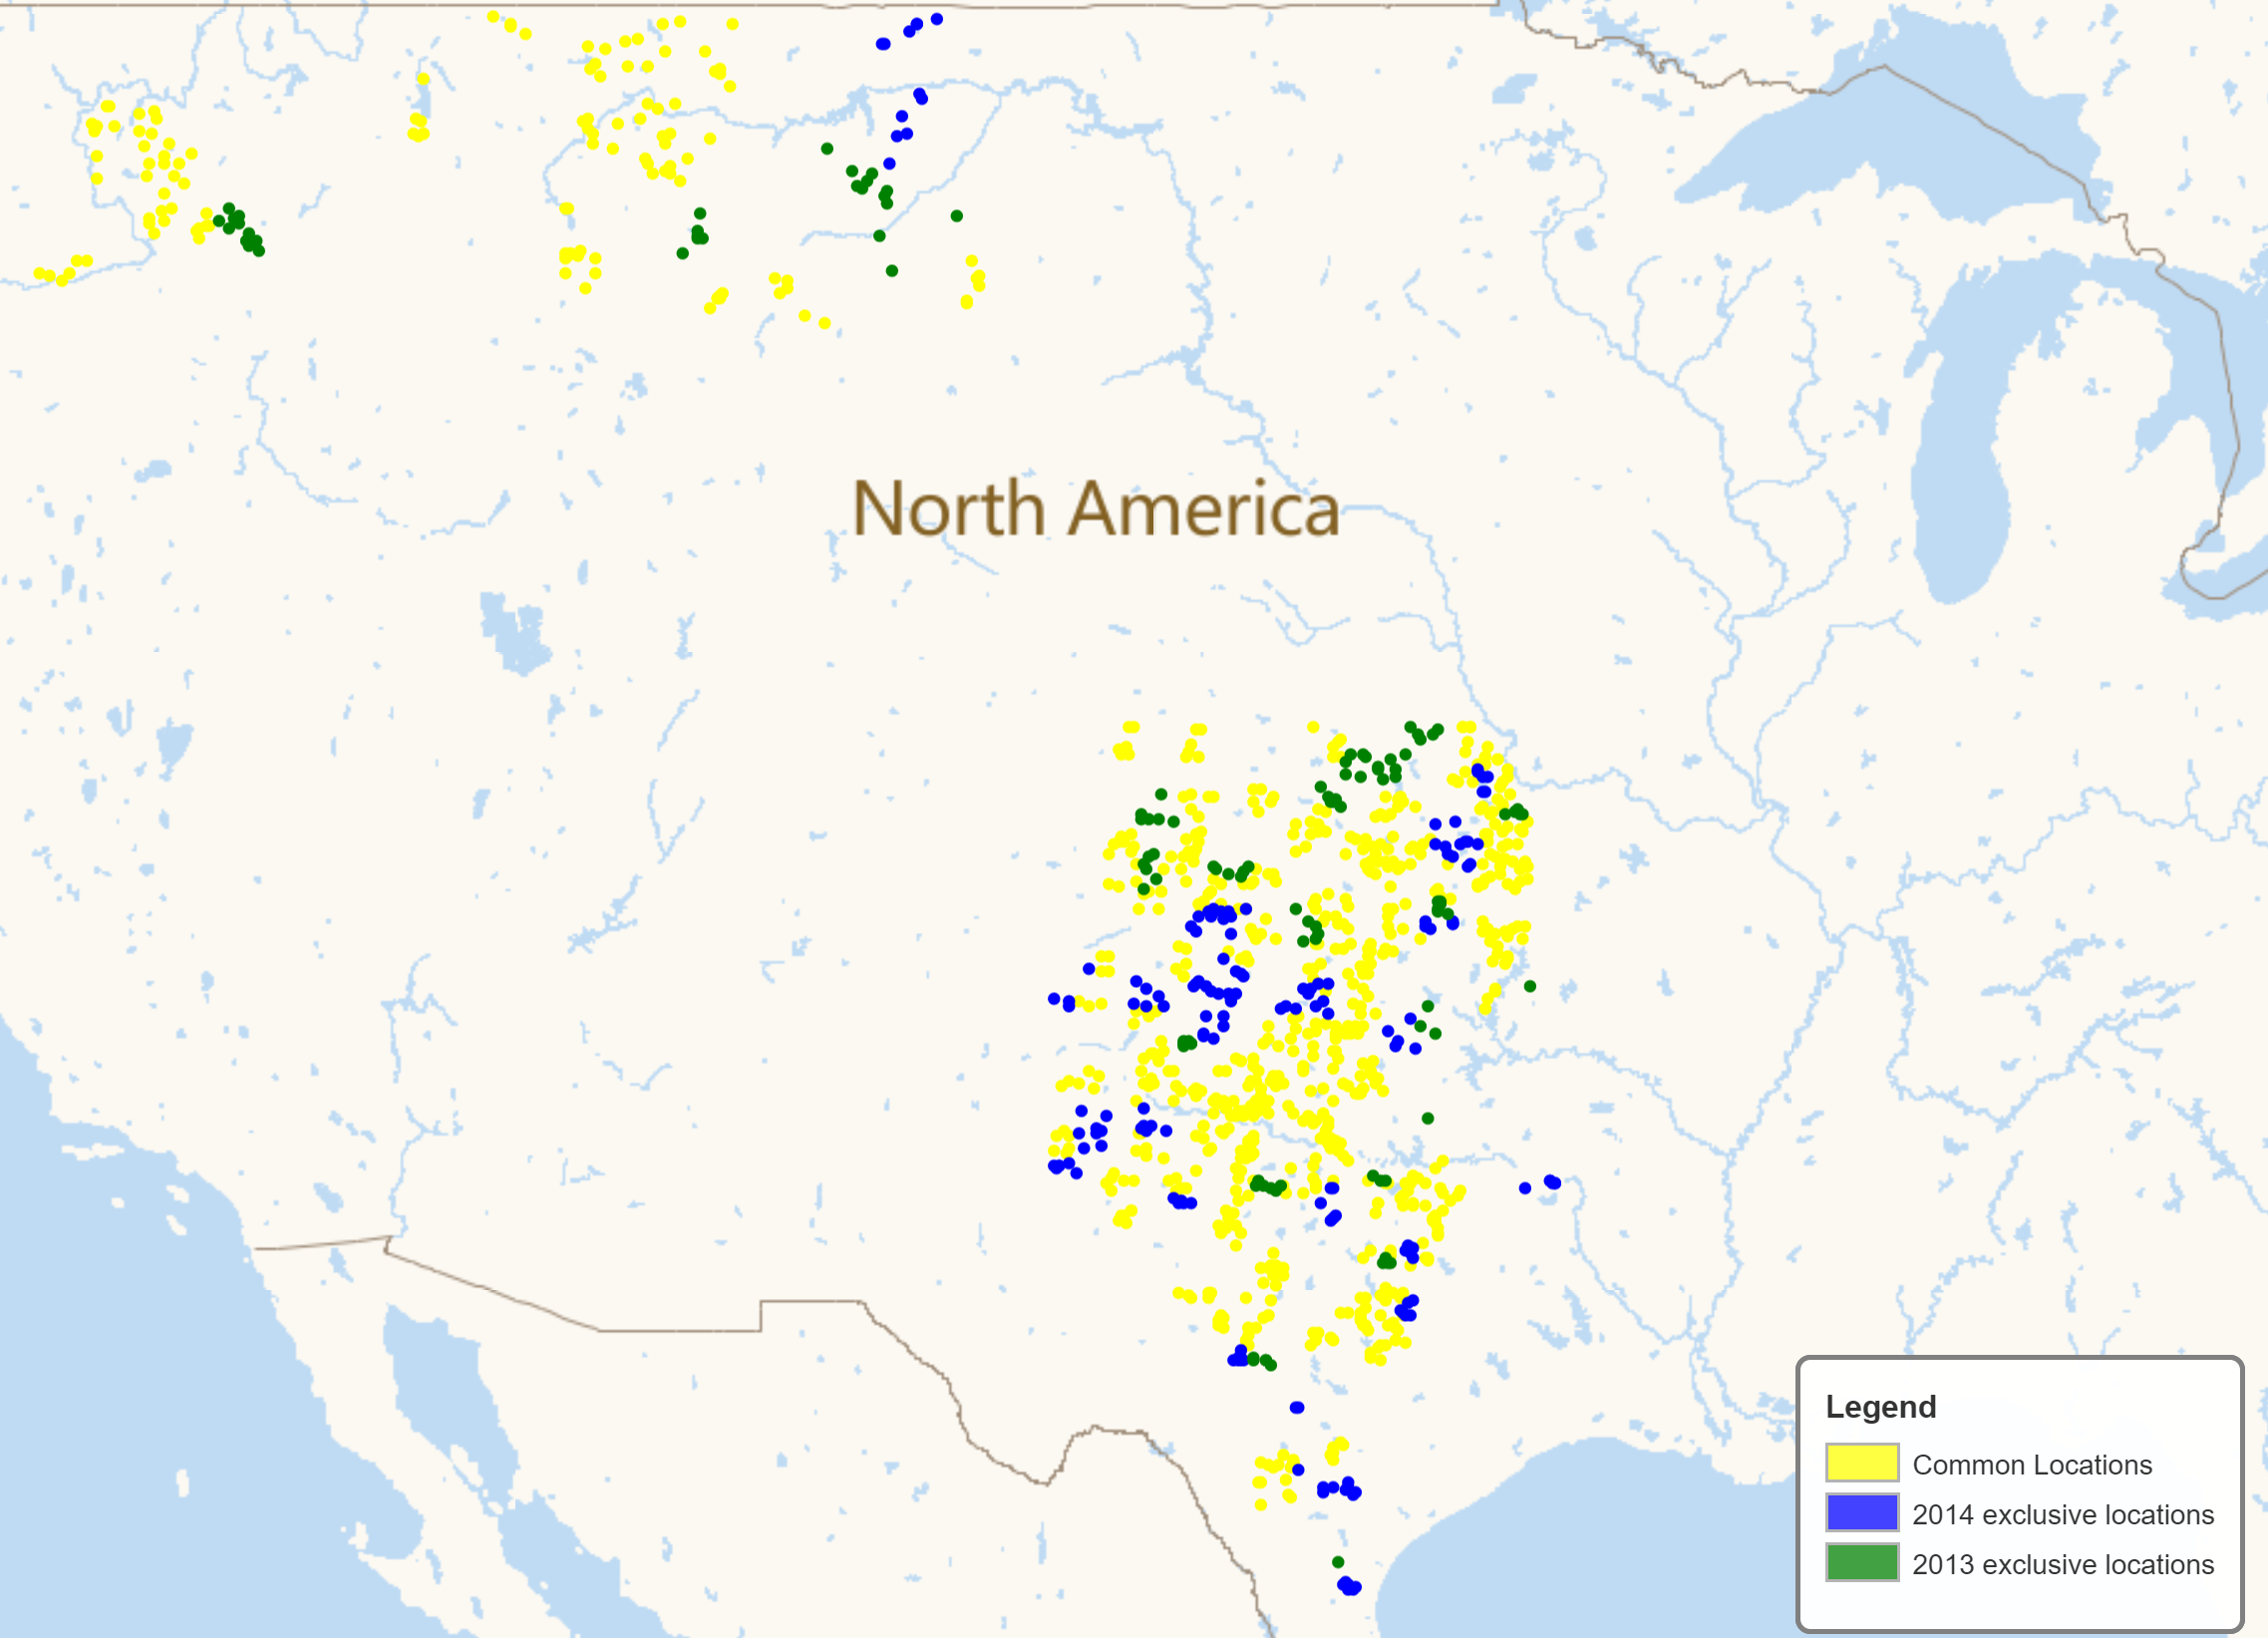
\includegraphics[width=0.45\linewidth]{./figures/data_locations.png}}
          \hfill
        \subfloat[\label{mapb}]{% TODO: replot figure 
              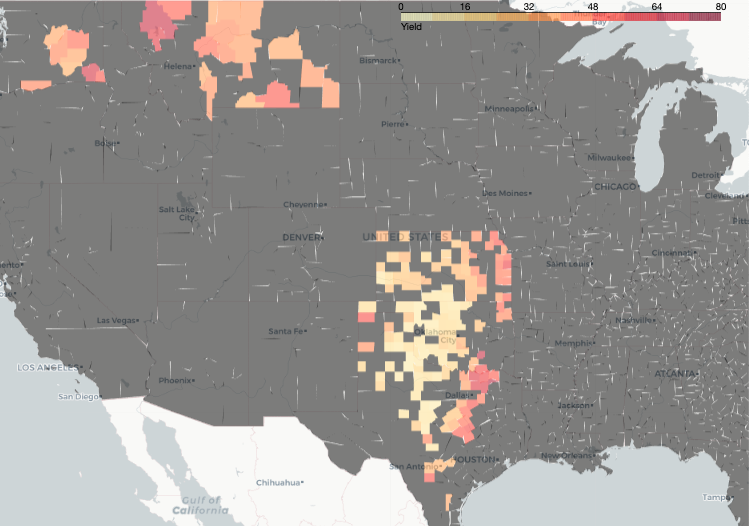
\includegraphics[width=0.45\linewidth]{./figures/map.png}}
        \label{fig:Map_visual} 
        \caption{(a)shows the location of all data being collected, yellow points represent locations monitored for two years which can be used for forecasting next year's yields via data of previous years. (b)shows the yield varying by locations}
      \end{figure*}

    \subsubsection{Feature selection}
      There is significant multicollinearity between some features in the data, which can lead to errors and distortions in the results\cite{farrar1967multicollinearity}. By calculating the correlation coefficient between the features, finding that there are features with a correlation higher than 90\% with another, some even reach 99\%. Table.~\ref{tab:correlation} shows the features correlation high than 90\%, these features accompanied with some other features unrelated to target such as \textit{State}, \textit{Date} e.t.
      \begin{table}[htbp]
        \caption{Features correlation high than 90\%}
        \begin{center}
          \begin{tabular}{|c|c|c|c|c|}
            \hline
            Feature 1 & Feature 2 & cor1 & cor2 & cor3\\
            \hline
            apparentTempMin & TempMin     & 0.99 & -0.04 & -0.06 \\
            apparentTempMax & TempMax     & 0.99 & -0.14 & -0.15 \\
            precipIntensity & precipIntensityMax & 0.91 & 0.04  & 0.03  \\
            dewPoint & tempMin & 0.91 & 0.01  & -0.06 \\
            apparentTempMin & dewPoint & 0.90 & -0.04 & 0.01 \\
            \hline
            \multicolumn{5}{l}{$^{\mathrm{a}}$cor1: correlation between feature1 and feture2} \\
            \multicolumn{5}{l}{$^{\mathrm{b}}$cor2: correlation between feature1 and yeild} \\ 
            \multicolumn{5}{l}{$^{\mathrm{c}}$cor3: correlation between feature2 and yeild} \\
          \end{tabular}
          \label{tab:correlation}
        \end{center}
      \end{table}




  \subsection{Bi-LSTM Model}
    \subsubsection{LSTM}
      Recurrent Neural Network is a kind of neural network that is good at processing time-series data. It can well process tasks with continuous-time and contextual relationships which is exactly in line with the characteristics of the crop growth. The connections existing between each layer make the network better in learning time series relations, but on the other hand, this leads to a gradient explosion in backpropagation. \cite{hochreiter1997long}

      \begin{figure}[htbp]
        \centerline{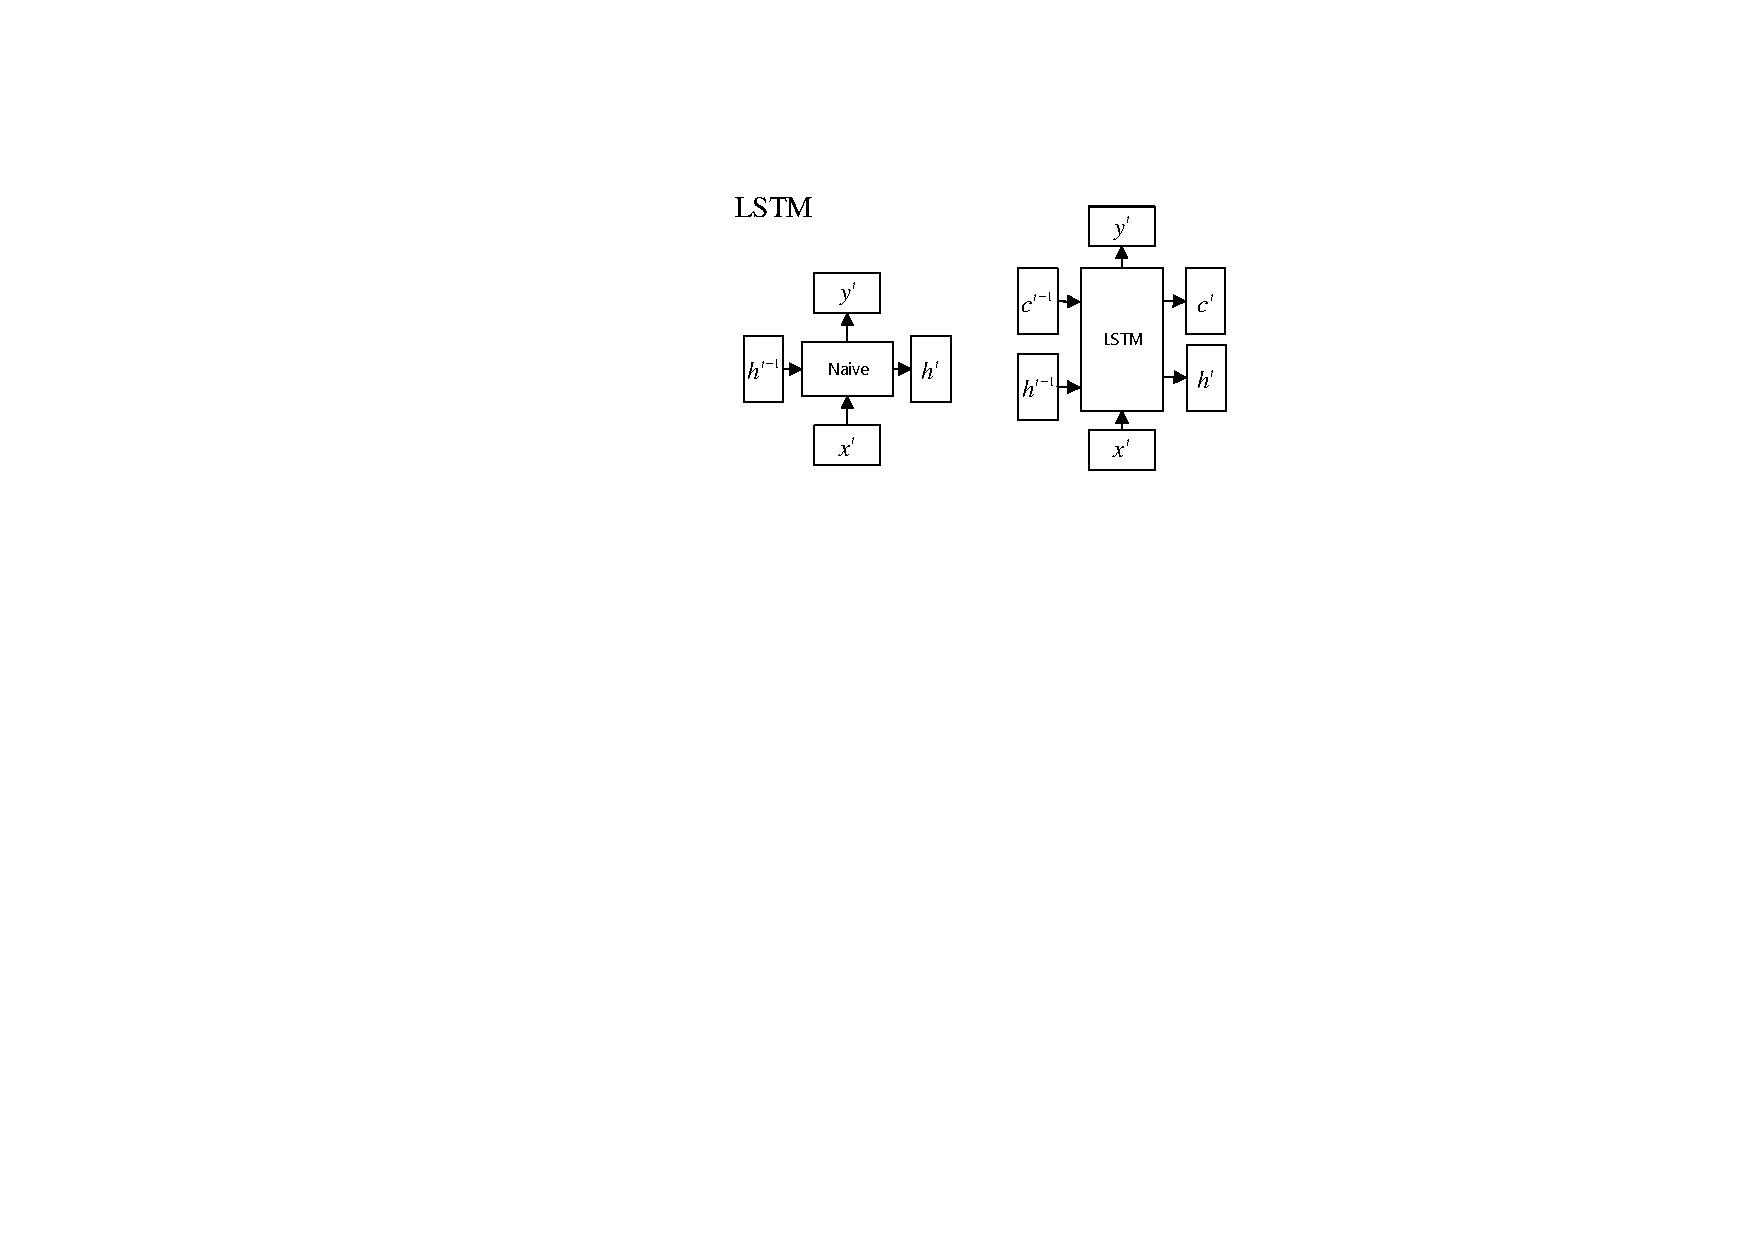
\includegraphics[width=0.7\linewidth]{figures/LSTM_struc.pdf}}
        \caption{LSTM and RNN structure}
        \label{fig:LSTM}
      \end{figure}

      Fig.~\ref{fig:LSTM} shows the structure of LSTM and RNN. The structure of t-th RNN node is on the first image, $x^t$ is the input of t-th node, $h^{t-1}$ is the input of t-th node received from $t-1$th node, $y^t$is the output and $h^t$ is the output which transfer to next node, while LSTM have two more states $c^t$(cell state) and $h^t$(hidden state), state $c$ in LSTM is the counterpart of state $h$ in RNN, and normally, state $c$ changes slowly in front propagation which typically to add a number to $c^{t-1}$. On the contrary, $h^t$ changes drastically.

      \begin{figure}[htbp]
        \centerline{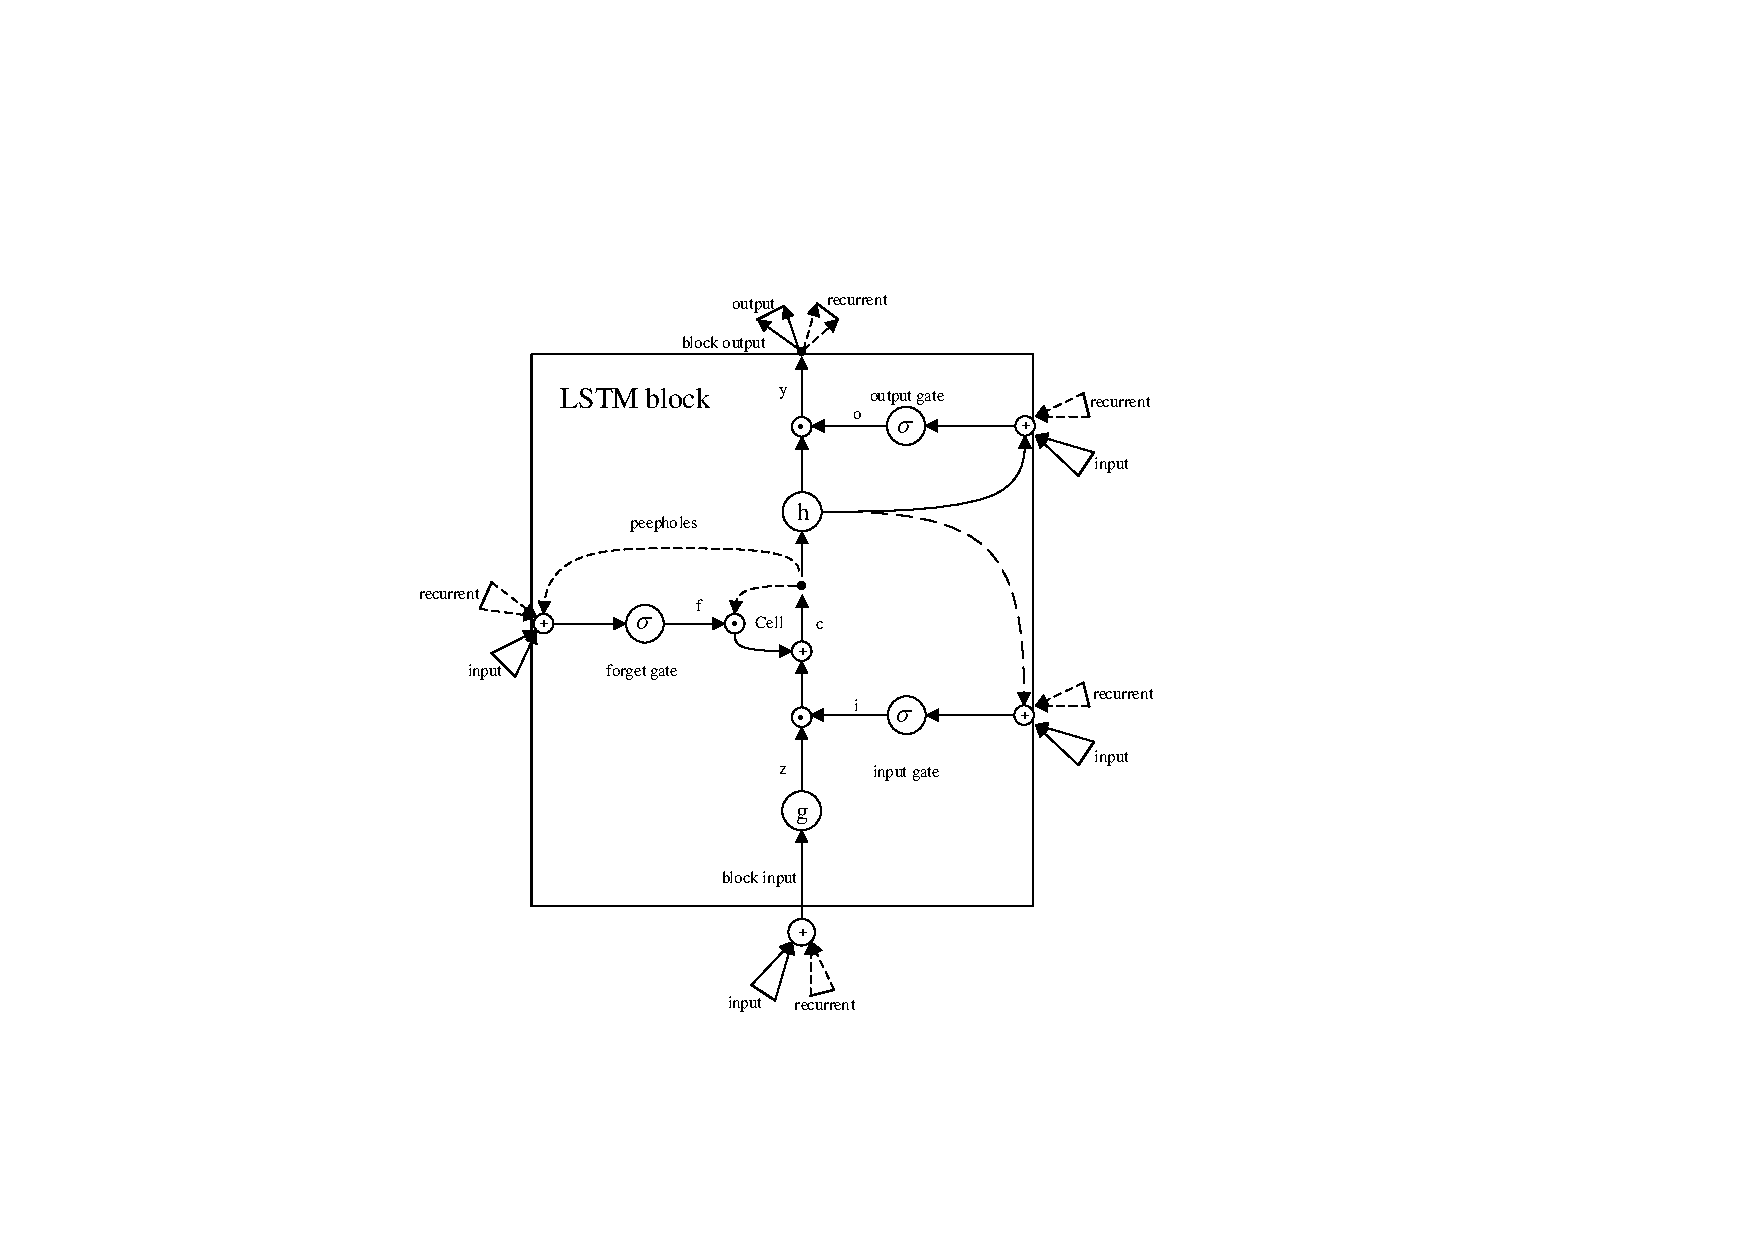
\includegraphics[width=0.7\linewidth]{figures/LSTM_node.pdf}}
        \caption{LSTM node}
        \label{fig:LSTM2}
      \end{figure}

      \begin{equation}
        \begin{cases}	f_t=\sigma \left( w_f\cdot \left[ h_{t-1},x_t \right] +b_f \right)\\	i_t=\sigma \left( w_i\cdot \left[ h_{t-1},x_t \right] +b_i \right)\\	o_t=\sigma \left( w_o\cdot \left[ h_{t-1},x_t \right] +b_i \right)\\\end{cases}
        \label{eq:gate}
      \end{equation}

      \begin{equation}
        \sigma \left( x \right) =\frac{1}{1+e^{-x}}
        \label{eq:sigmoid}
      \end{equation}
      For a LSTM node shown in Fig.~\ref{fig:LSTM2}, four states $f_t$(forget gate), $i_t$(input gate), $c_t$(current state) and $o_t$(output gate) are generated by concating $x^t$ and $h^{t-1}$ via (\ref{eq:gate}). Forget gate $f_t$ control the remain of information transtered from $c_{t-1}$, $[h_{t-1}, x_t]$  means to concat vector $h_{t-1}$ and vector $x_t$, $w_f$ and $b_f$ are the weight and bias of forget gate $f_t$, $\sigma$ is the Sigmoid activate function, expression of Sigmoid is (\ref{eq:sigmoid}).



      To calculate $c_t$, the input state $\widetilde{c_t}$ are needed to be calculate first. Use activate function $\tanh$ via (\ref{eq:ct1}), (\ref{eq:ct2}) and (\ref{eq:gate}) to calculate $c_t$, the $\odot$ in (\ref{eq:ct2}) means corresponding element multiplication.

      \begin{equation}
        \tilde{c}_t=\tanh \left( W_c\cdot \left[ h_{t-q},x_t \right] +b_c \right)
        \label{eq:ct1}
      \end{equation}

      \begin{equation}
        c_t=f_t\odot c_{t-1}+i_t\odot c_t
        \label{eq:ct2}
      \end{equation}

      All these features of LSTM meet the crop growing process, there are weather fluctuations or natural disasters in a short time, while there are stable natural conditions over a long period..

    \subsubsection{Bi-LSTM Model}
      As shown in Fig.~\ref{fig:model}, build a Bi-LSTM network using Keras and Tensorflow, there are two parts in the model. The left part is three layers of stacked Bi-LSTM use to predict the yield by the weather data, right part use stacked fully connected network to link the county and the predicted yield.

      \begin{figure}[htbp]
        \centerline{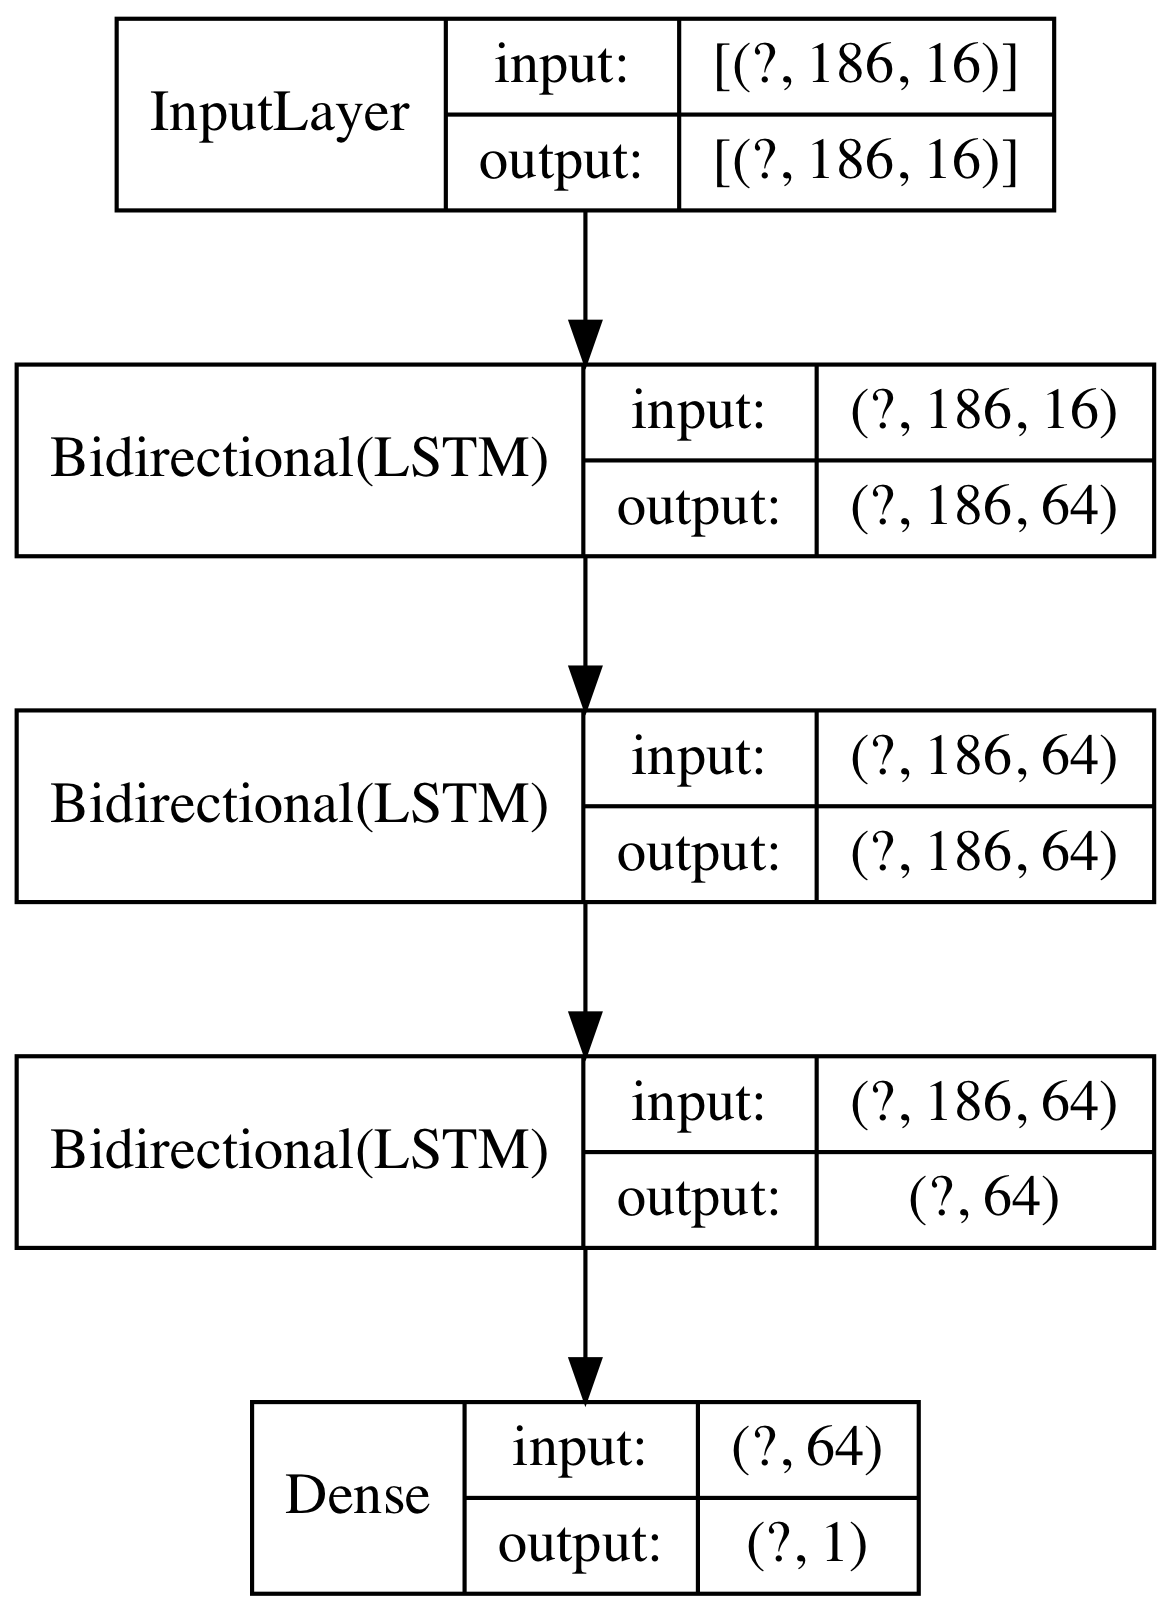
\includegraphics[width=0.4\linewidth]{figures/Model_figure.png}}
        \caption{Bi-LSTM Model}
        \label{fig:model}
      \end{figure}


\section{Experiment} \label{sec:ex}
\subsection{Test method}
  Before testing, use the \textit{Min-Max} method shown by (\ref{eq:standarlize}) to standardize data and shuffle data due to the data is arranged by location. If not doing so, there will be data from new locations in train data while splitting the test set and train set.

  \begin{equation}
    x_i := \frac{x_i-\min \left( x_i \right)}{\max \left( x_i \right) -\min \left( x_i \right)}
  \label{eq:standarlize}
  \end{equation}

  Because the time complexity of SVR is more than twice the data size\cite{clarke2005analysis}, extract 10000 entries of data to reduce time, randomly extract, and run multiple times to avoid accidental exceptions caused by extraction.



\subsection{Test Result}
  The result of the algorithm test is as shown in Table.~\ref{tab:result} and RF shows severe overfitting among all the algorithms. The prediction contribution of features shown in Table.~\ref{tab:RF_contribution}, it is obvious that yield prediction is dominated by location.

  \begin{table}[htbp]
    \caption{Performance of algorithms on crop yield prediction}
    \begin{center}
    \begin{tabular}{|c|c|}
    \hline
    Algorithm                                    & MSE      \\
    \hline
    Random Forest \cite{liaw2002classification}                               & 0.0048   \\
    Random Forest(10K)                           & 0.1096   \\
    KNN \cite{peterson2009k}                                         & 60.6555  \\
    Polynomial regression  \cite{theil1992rank}                      & 108.4011 \\
    Polynomial regression with L2 regularization & 108.4891 \\
    Linear regression \cite{vapnik2013nature}                           & 179.4249 \\
    Linear regression with L2 regularization     & 179.4339 \\
    SVR(1K) \cite{drucker1997support}                                     & 188.4630 \\
    SVR RBF kernel(10K) \cite{cristianini2000introduction}                         & 193.5149 \\
    SVR linear kernel(10K) \cite{cristianini2000introduction}                      & 197.0644 \\
    Gradient boost \cite{ke2017lightgbm}                              & 231.4852 \\
    KRR  \cite{saunders1998ridge}                                        & 333.6586 \\
    \hline
    \multicolumn{2}{l}{$^{\mathrm{a}}$ 10K: Extract 10K entries of data to reduce training time} \\
    \end{tabular}
    \label{tab:result}
    \end{center}
  \end{table}

  \begin{table}[htbp]
      \caption{Feature contribution of RF}
      \begin{center}
      \begin{tabular}{|c|c|}
      \hline
        Feature & Contribution \\
      \hline
        Longitude & 0.7656 \\
        Latitude & 0.2342 \\
        cloudCover & 0.0001 \\
      \hline
      \end{tabular}
      \label{tab:RF_contribution}
      \end{center}
  \end{table}

  Group the data by location and check the yield finding that the number of unique yields does not match that of locations, which means there are entries share the same yield. Look further into data, finding that the yield of a day is not the real yield of the current day, but the yield of final yield. What's more, the locations from the same county also share the same yield. That directly results in locations' neighborhoods get the same yields, and the algorithm can give the exact yield according to the yield.  

\subsection{Overfitting in Random Forest}
  Simply remove longitude and latitude form data and run the test again, get the learning curve shown by Fig.~\ref{cv1}. It is not the "location" leads to the overfitting, but the structure of data.

  \begin{figure}[!htb]
    \centering
  \subfloat[\label{cv1}]{%
      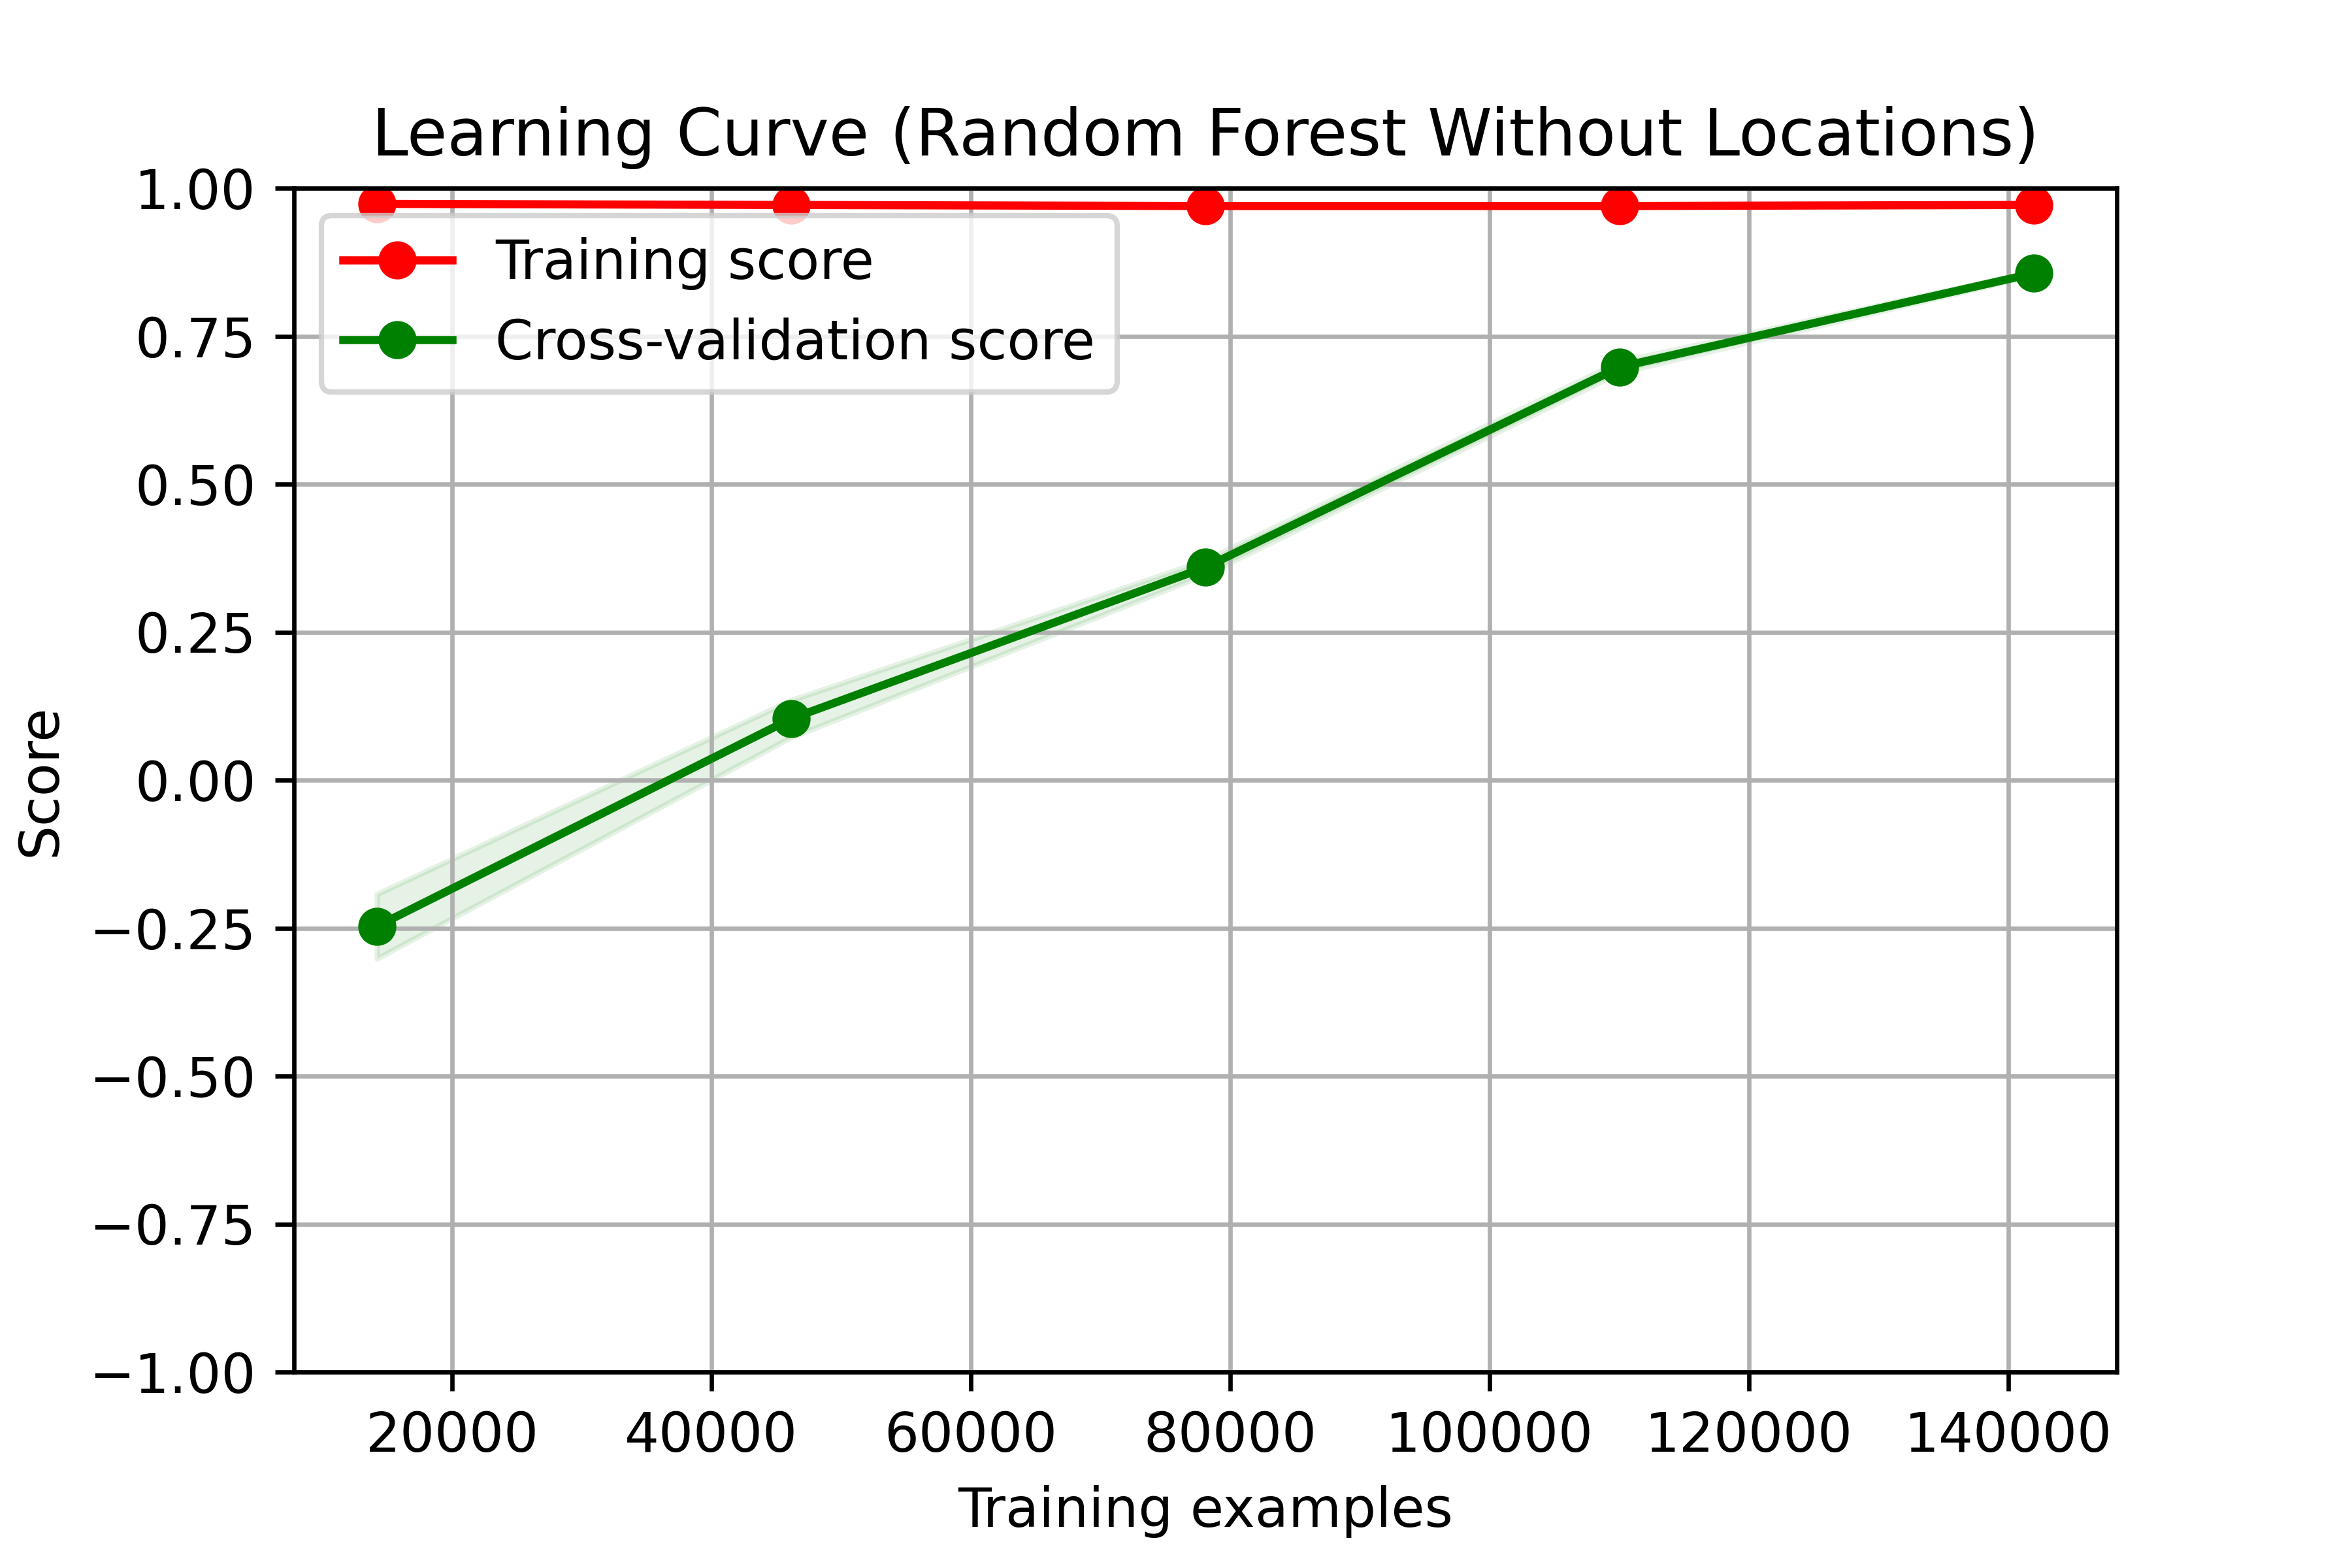
\includegraphics[width=0.5\linewidth]{./figures/Learing Curve1.png}}
  \subfloat[\label{cv2}]{%
        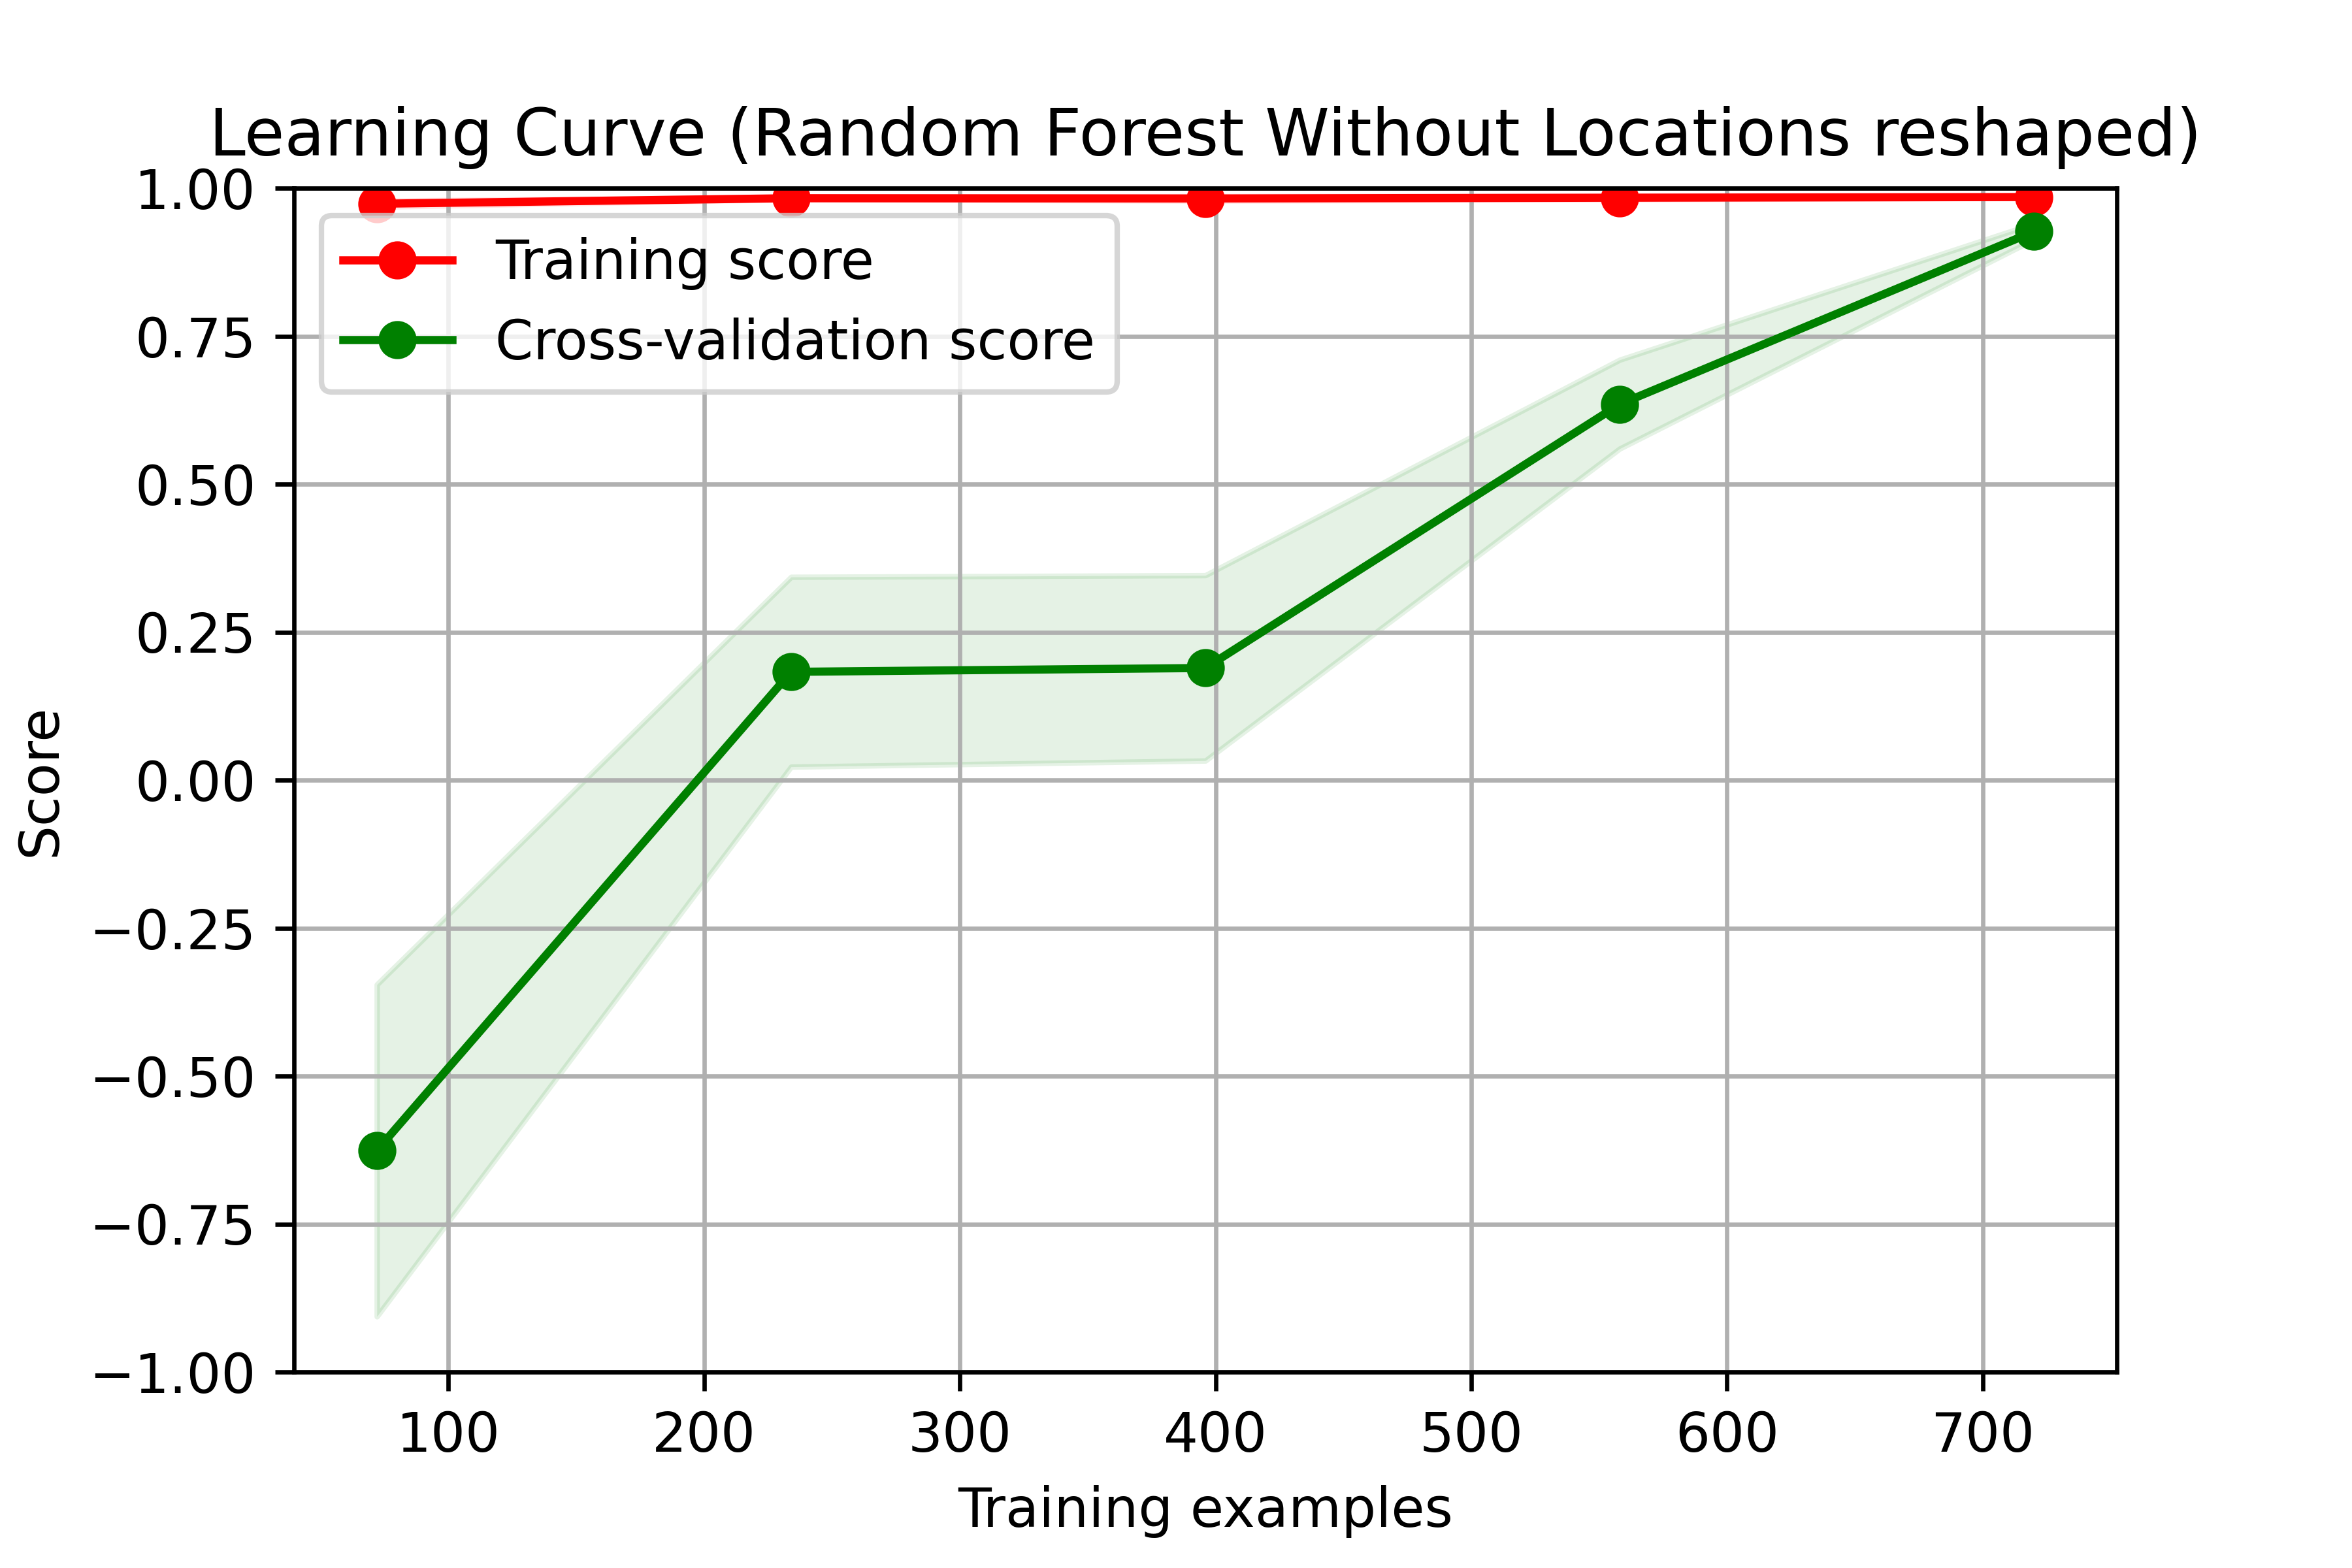
\includegraphics[width=0.5\linewidth]{./figures/Learing Curve2.png}}
  \hfill
  \subfloat[\label{cv3}]{%
        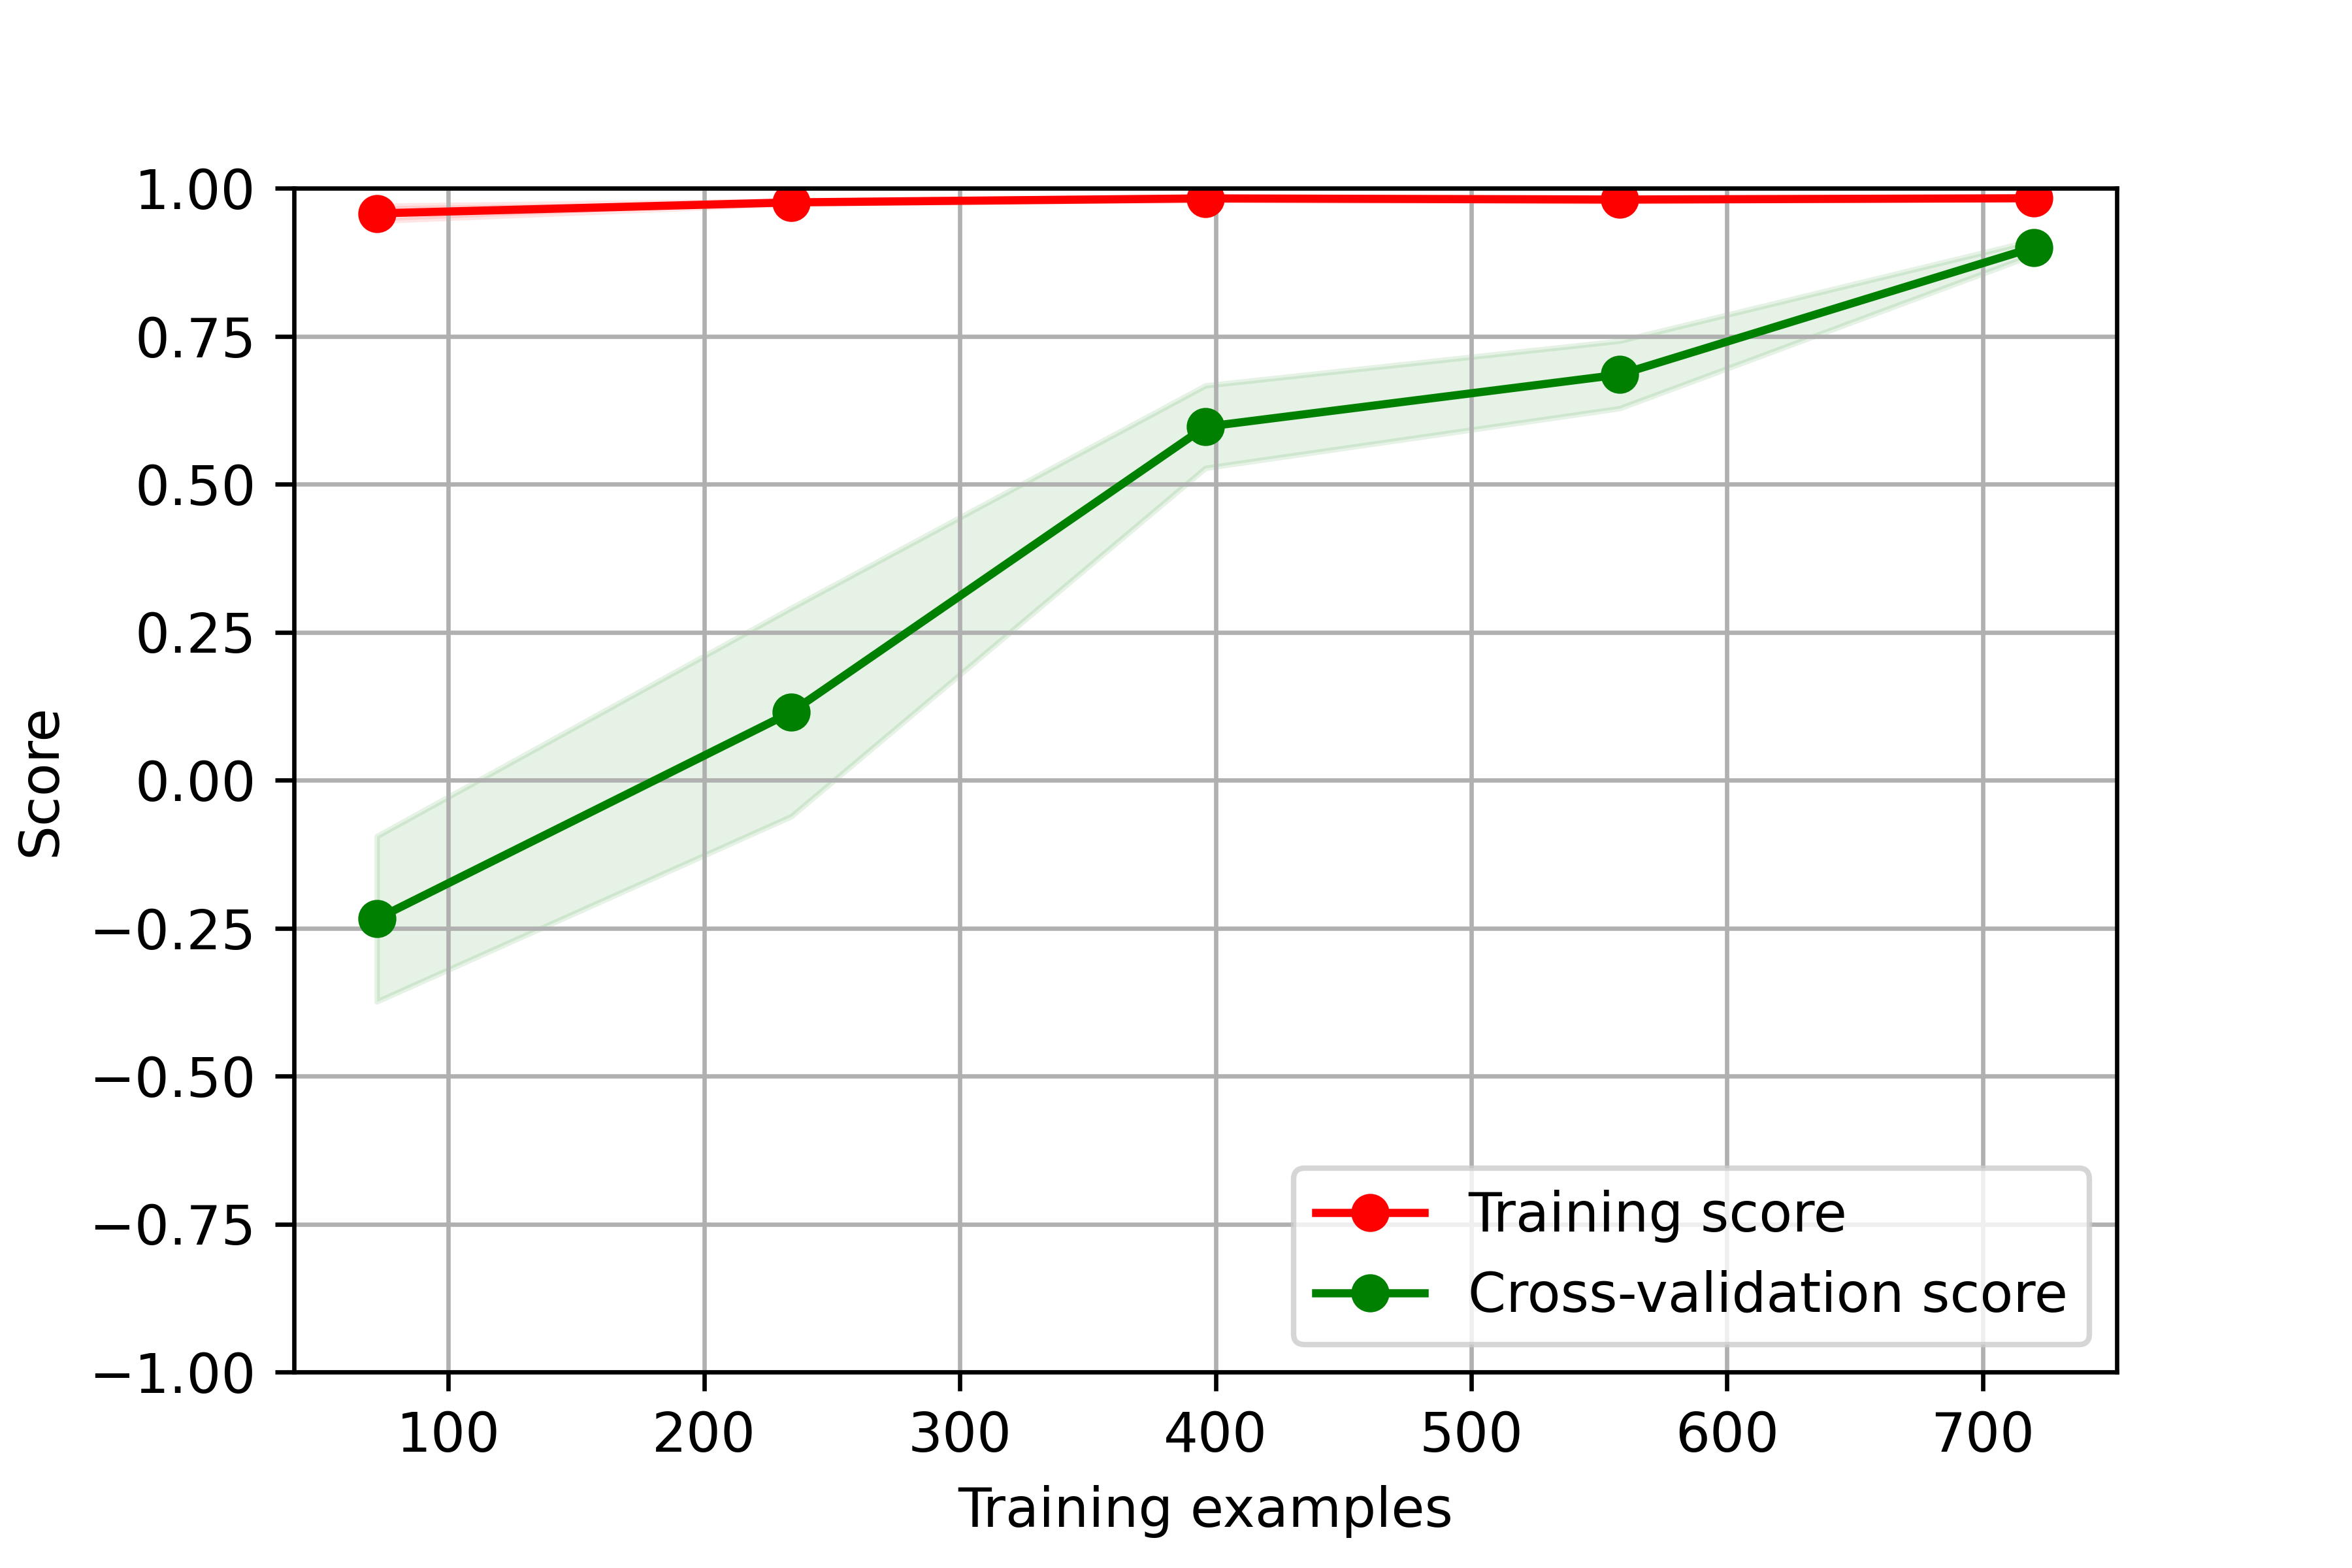
\includegraphics[width=0.5\linewidth]{./figures/Learing_Curve3.png}}
  \subfloat[\label{cv4}]{%
        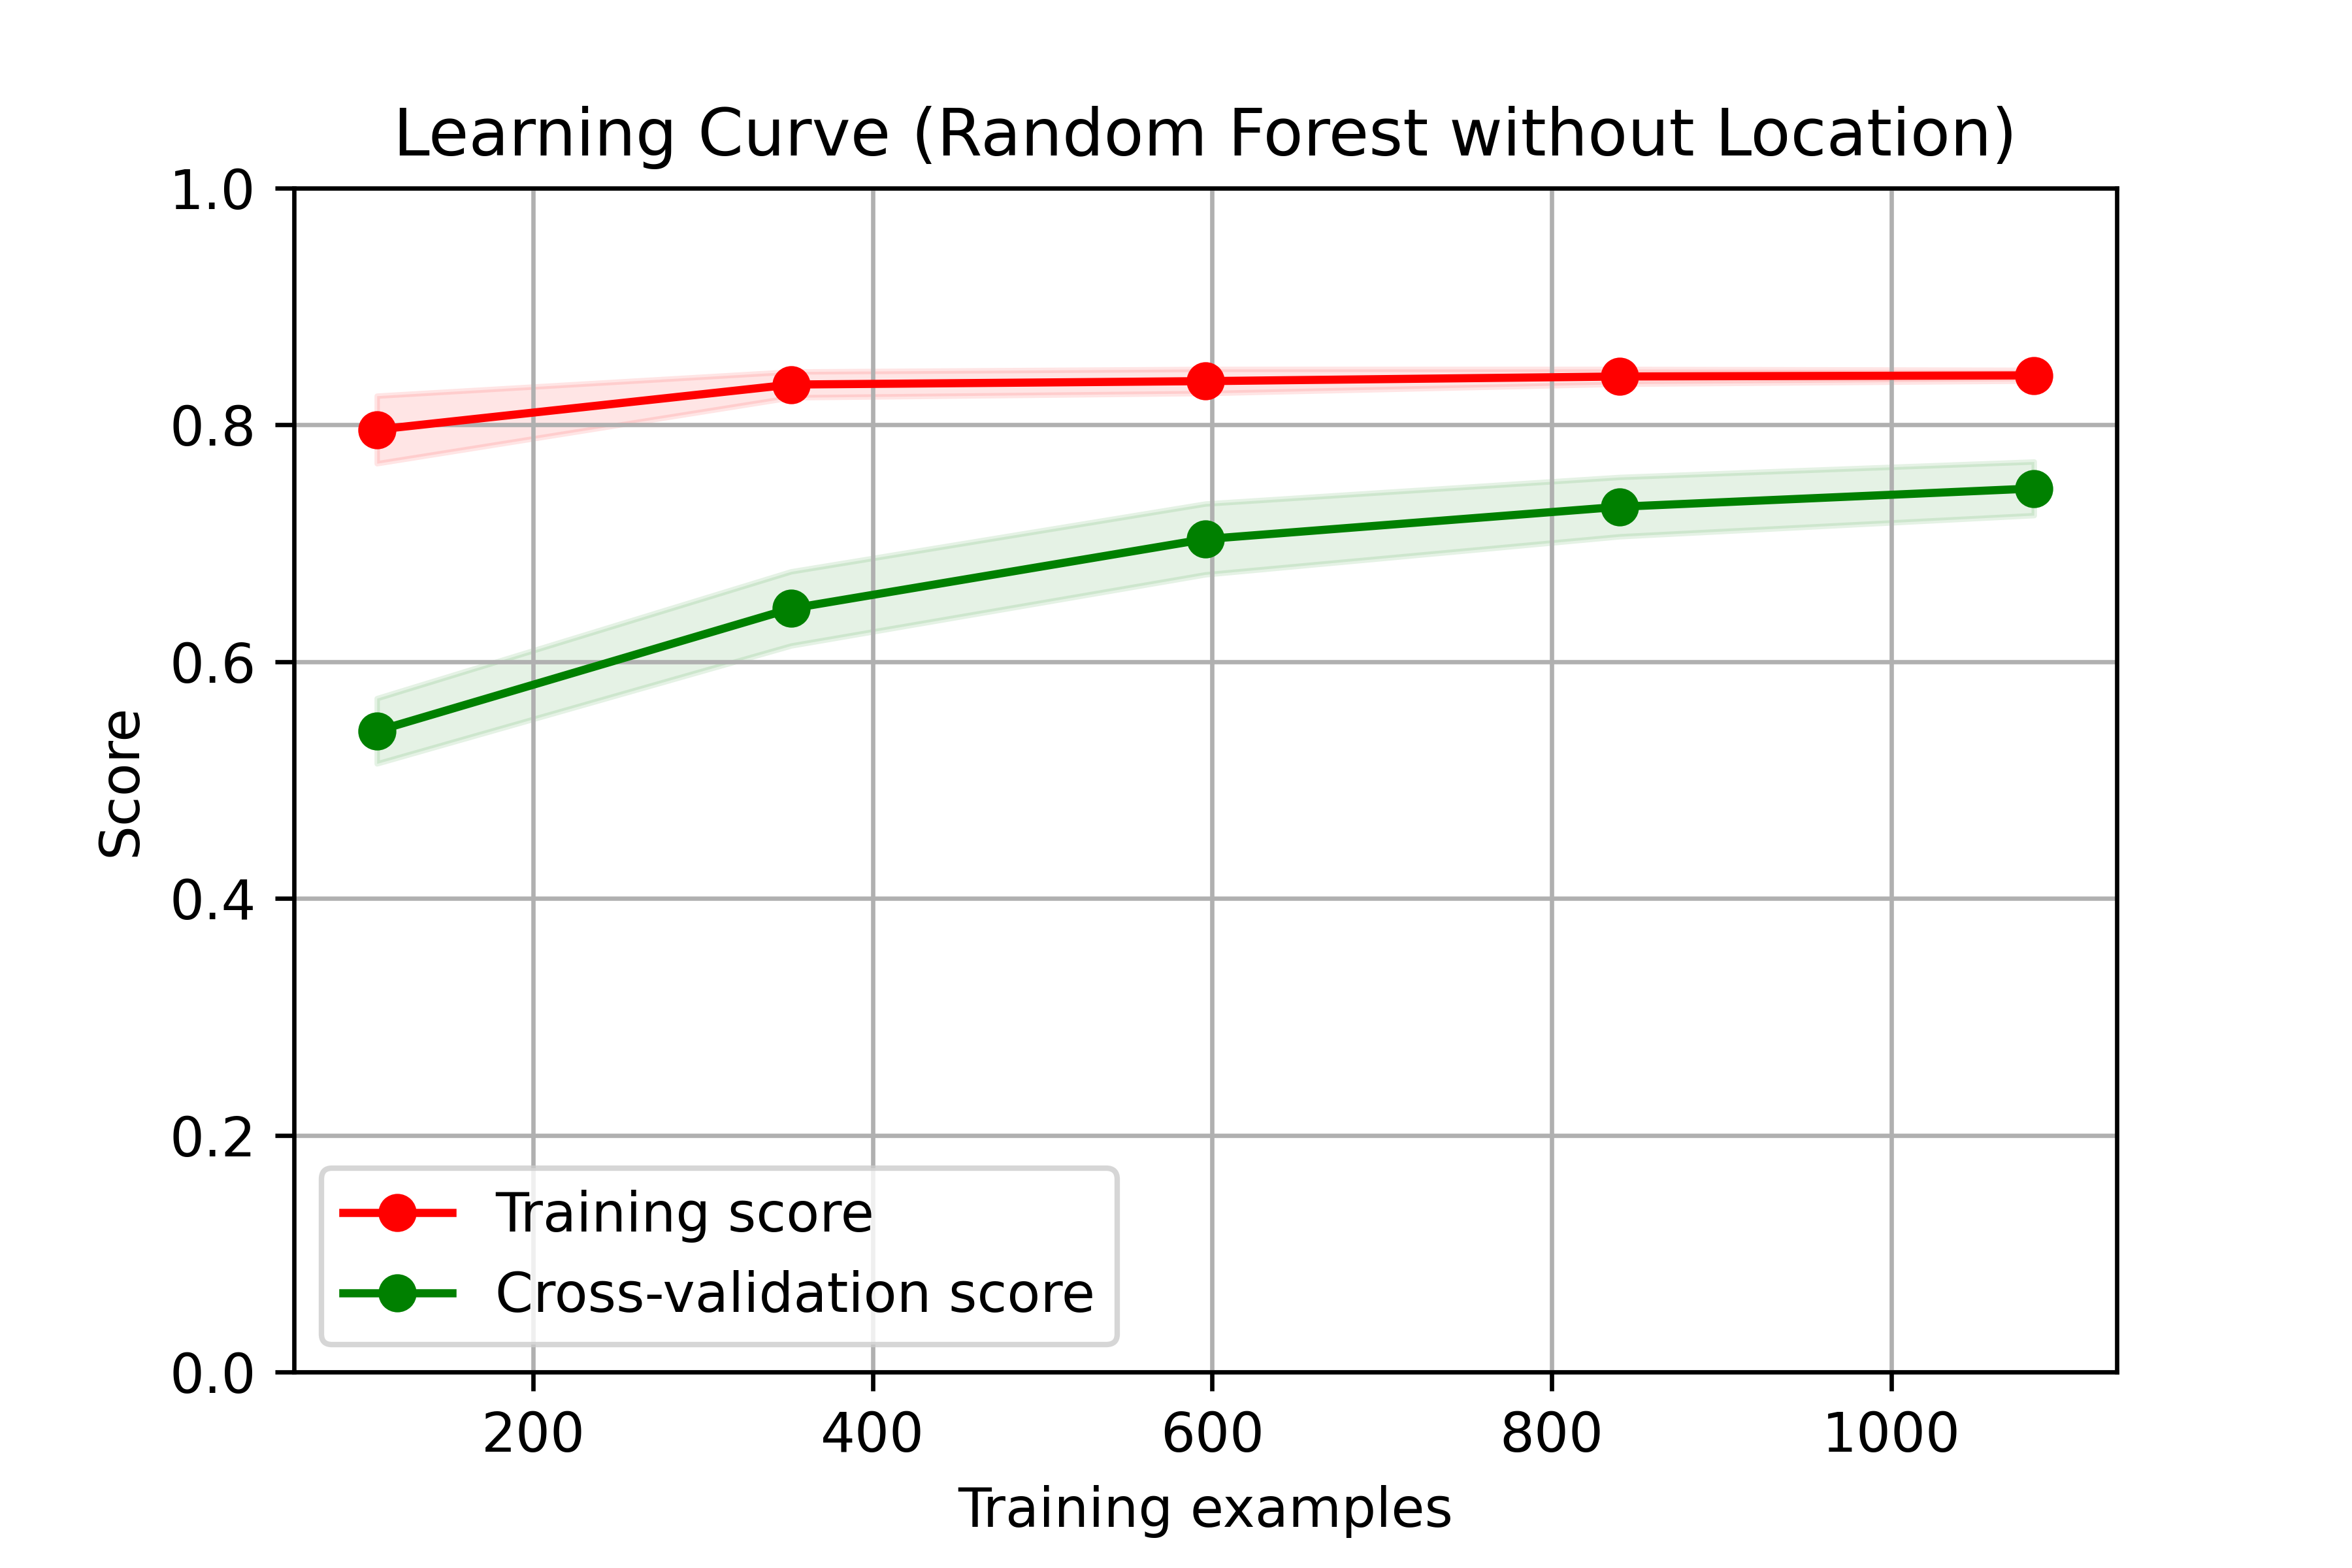
\includegraphics[width=0.5\linewidth]{./figures/cv4.png}}
  % \label{fig:lc} 
    \caption{Learning Curve of Random Forest. (a) generated by the origin data, obviously, there's severe overfitting. (b) generated by setting data of different days to a new feature, performance gets worse. (c) generated by compress the data, the CV-score gets better. (d) generated by feature selection, the overfitting problem being solved}
  \end{figure}

  Reshape data to shrink the disparity between yield and data entries. For data in 2013, the original shape is $(166685,16)$, which means that there are 186 days every location for 16 features. Transform the shape of data into $(901\times2960)$ and run the test again to get the learning curve shown in Fig.~\ref{cv2}. These two methods can't solve the overfitting problem.

  Try to aggregate the data to shrink the number of features. Calculate the mean values of ever 60 days and shrink features to 48, run the test again, and get the learning curve shown in Fig.~\ref{cv3}. There is some improvement after half of the dataset getting involved.

  To extract some indirect features from the origin features, we calculate the minimum and maximum value of features in 30 days, minimum maximum NDVI in 30 days, mean temperature difference, and variance e.t using a rolling window method from pandas. Then, run the test base on these indirect features get the learning curve in Fig.~\ref{cv4}.

\subsection{LSTM}
  Use the EarlyStopping callback function to alleviate overfitting and set training epoch to 1000. The process of training shown in Fig.~\ref{fig:train}.

  \begin{figure}[htbp]
    \centerline{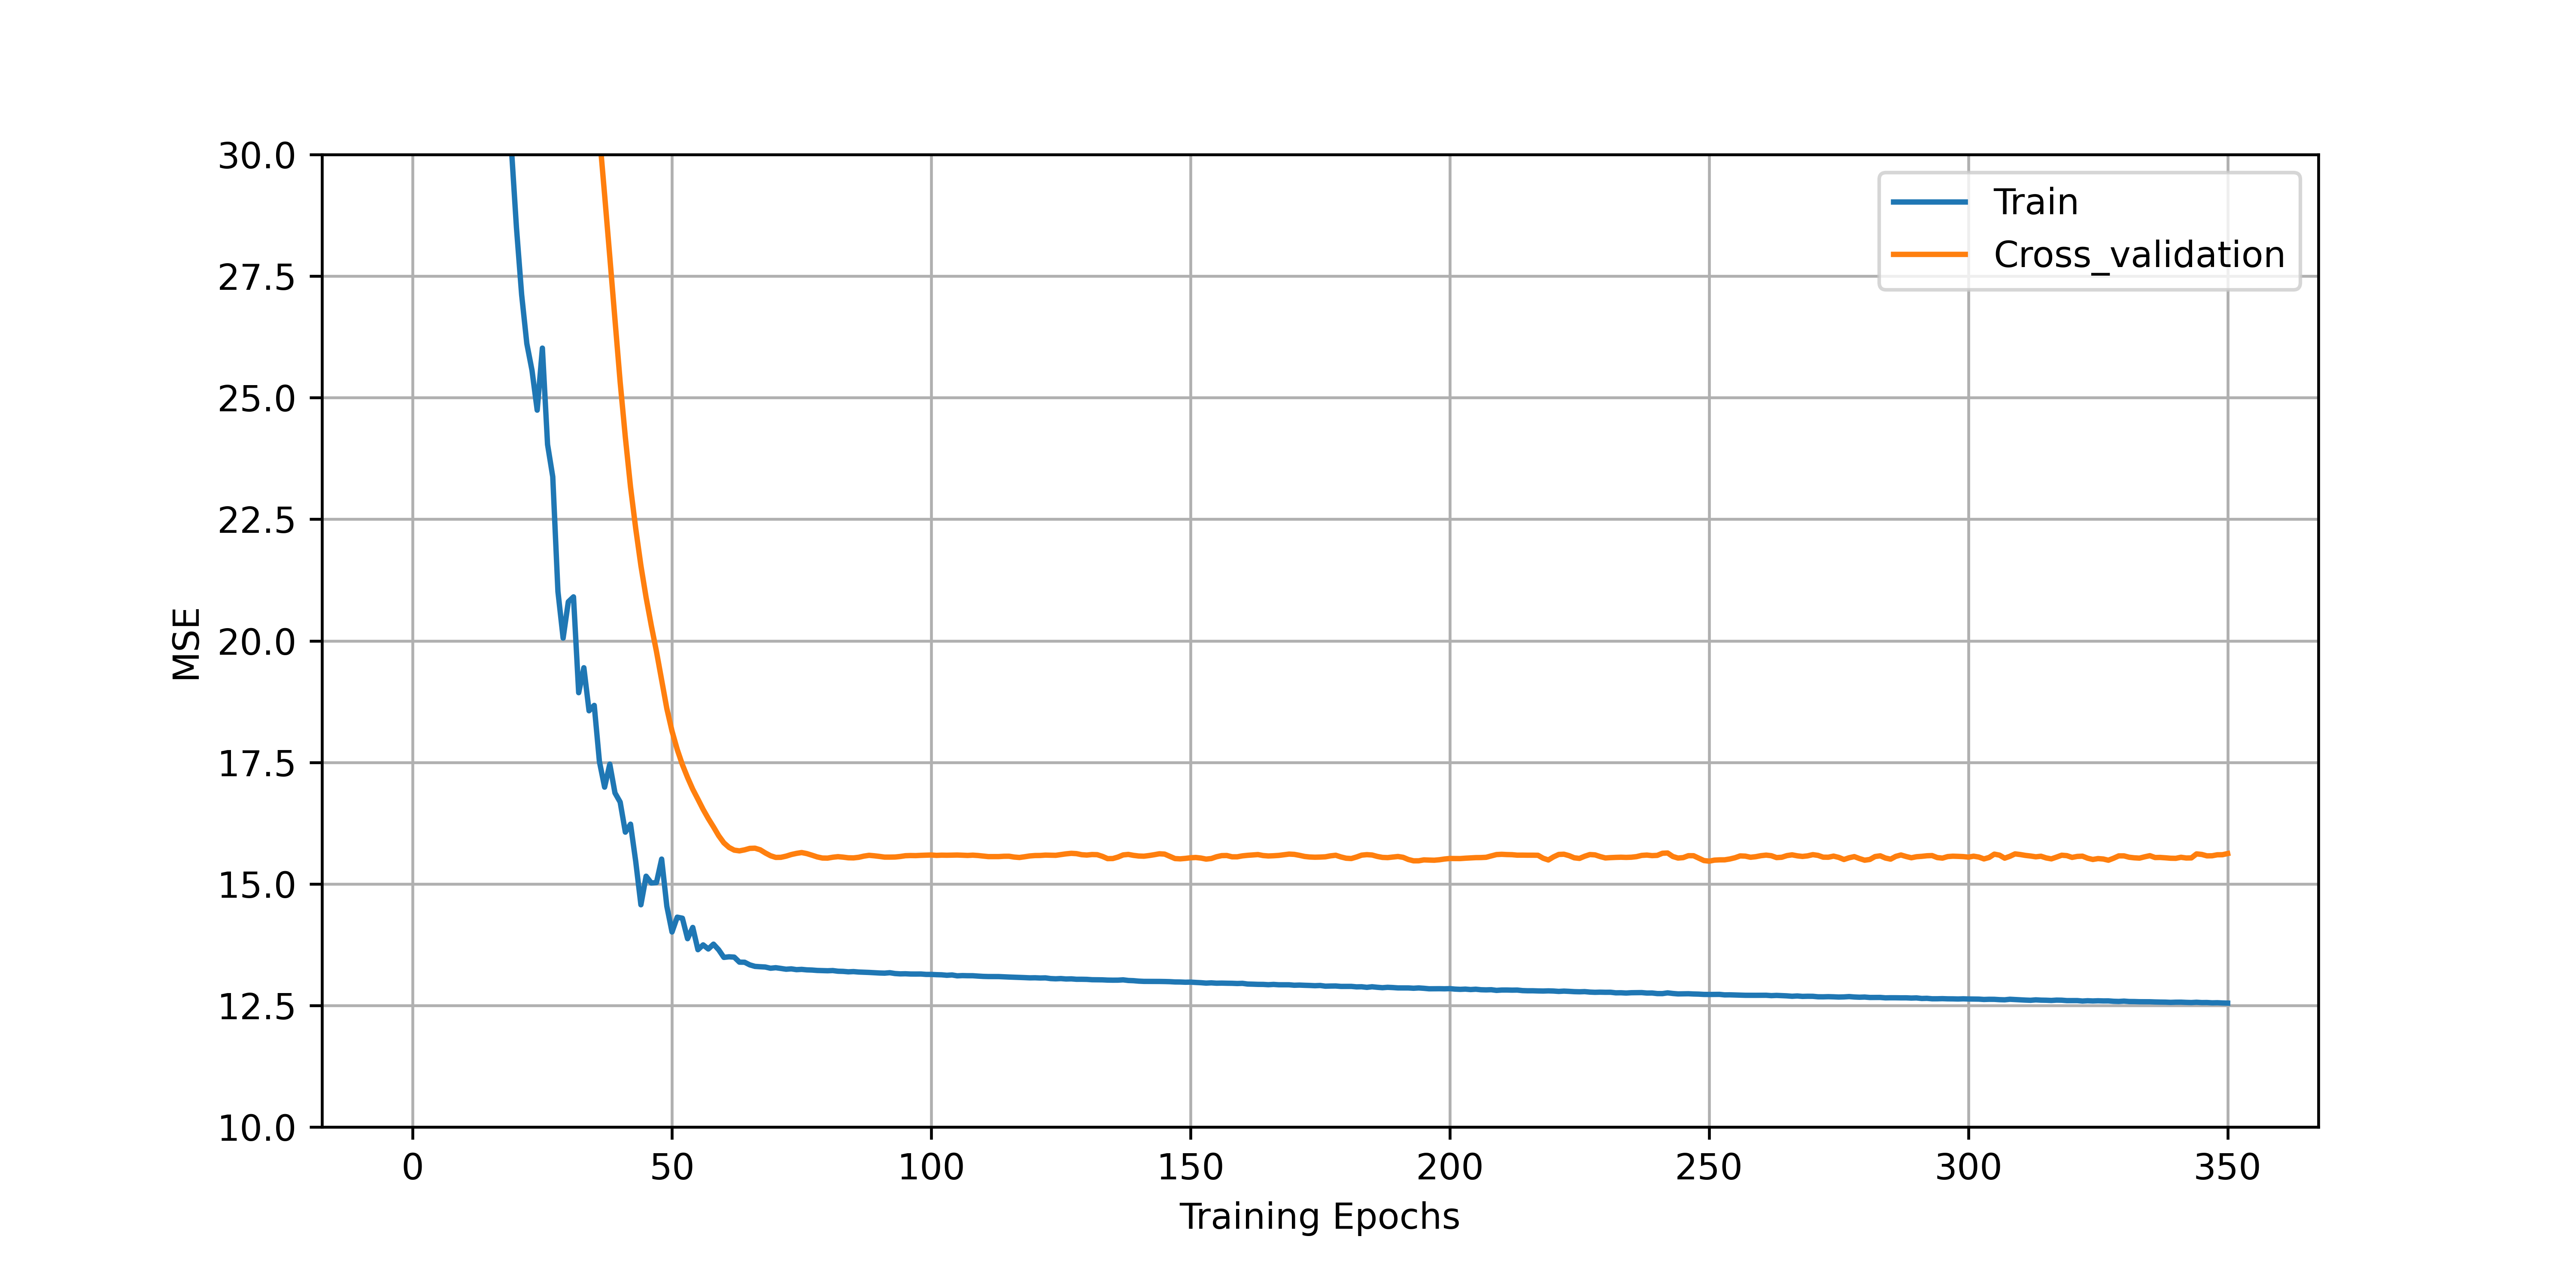
\includegraphics[width=\linewidth]{figures/lp.png}}
    \caption{Training Process of LSTM}
    \label{fig:train}
  \end{figure}

  The MSE of both training and cross-validation go lower accompanied by the increment of training epochs. This procedure has been run several times, it always triggers the EarlyStopping callback function at between 100 to 300 epochs. The final mean cross-validation MSE for all runs is 12.3793 comparing to RF's 23.72, the performance of LSTM is 47.84\% better than RF which is quite accurate to forecast the yield of corps whose $R^2$ error is 83.61\% after solving the overfitting problem.

\section{Conclusion and Future work} \label{sec:con}
  We composed a Bi-LSTM model to predict the wheat yield in the U.S and compared it with some commonly used regression algorithms. The results show that the model outperforms all of the algorithms this paper involveed and less likely to get overfitting which is commonly found in other regression algorithms. However, there are still some factors we do not consider due to the limitation of data. Some features which are crucial to the growth of crops, such as how farmers plant the crop and the condition of the sow in a certain location e.t, are not involved in the models due to the lack of data sources. The weather, undoubtedly, greatly influence the yield of corps, but some subjective behaviors of human can also influence the yield. The corps is not planted in an environment free of human intervention, water the crops when precipitation is a bisic natural behavior that people influence the planting. If can get access such sort of data, the accuracy of prediction will be higher. 

\bibliographystyle{IEEEtran}
\bibliography{IEEEabrv,reference}

\end{document}
